\documentclass[10pt]{article}

%%%%%%%%%%%%%%%%%%%%%%%%%%%%%%%%%%%%%%%%%
%%%%%%%%%%%%%% TYPOGRAPHIE %%%%%%%%%%%%%%
%%%%%%%%%%%%%%%%%%%%%%%%%%%%%%%%%%%%%%%%%

%%%%%%%%%%%%%% TEXT
    \usepackage{polyglossia} %| Für deutsche Sprache & Sonderzeichen
    \setmainlanguage{german} %| 
    \usepackage{microtype} % Für schöneren Blocksatz
    % \baselineskip = 30pt
    \usepackage[skip=4pt]{parskip} % Für "deutche" Absätze
    \usepackage[official]{eurosym} % Für Eurozeichen
    \usepackage[locale=DE, per-mode=symbol]{siunitx} % Für Einheiten
    \DeclareSIUnit{\dek}{Dekade}
    \DeclareSIUnit{\eur}{\mbox{\euro}}
    \usepackage{fontspec}
    % https://tex.stackexchange.com/questions/25249/how-do-i-use-a-particular-font-for-a-small-section-of-text-in-my-document/37251#37251
    \newfontfamily\sansemph{Latin Modern Sans} % Für Titel
    \usepackage{csquotes} % Für deutsche Anführungszeichen
    \newcommand{\form}[1]{#1} % Formeln
    \newcommand{\filepath}[1]{\texttt{#1}}
    \newcommand{\cmd}[1]{\texttt{#1}}
    \newcommand{\eng}[1]{\textit{#1}}
    \newcommand{\feng}[1]{{#1}}

%%%%%%%%%%%%%% MATHE
    \usepackage{amsmath} %| Standard ams packages
    \usepackage{amssymb} %|
    \usepackage{amstext} %|
    \newcommand{\sig}{\textrm{sig}}
    % \newcommand{\tanh}{\textrm{tanh}}
    \newcommand{\netin}{\textrm{net}}
    \usepackage{mathtools} % \xRightarrow

%%%%%%%%%%%%%% TEXTLAYOUT
    \usepackage{geometry} % Für Anpassung der Seitenränder
    \geometry{
    	top=2.5cm,
    	left=2.5cm,
    	right=2.5cm,
    	bottom=2cm,
    	% footskip=13.6pt
    }
    \usepackage{fancyhdr} % Kopf- und Fußzeilen
    % \pagestyle{plain}{
    % \fancyhf{}
    % \fancyhead[R]{JUGEND FORSCHT -- PROJEKTBERICHT}
    % }
    % \fancyfoot[C]{\thepage}
    
\renewcommand{\subsectionmark}[1]{%
  \markright{\MakeUppercase{\thesubsection.\ #1}}}%
\renewcommand{\sectionmark}[1]{%
  \markright{\MakeUppercase{\thesection.\ #1}}}%
% \renewcommand{\subsubsectionmark}[1]{%
%  \markright{\MakeUppercase{\thesubsubsection.\ #1}}}%
    \usepackage{multicol} % Text in mehreren Spalten
    \newcommand{\threesub}[1]{
        \vspace{1.5ex}
        \noindent {\textbf{#1}}
        \vspace{0.5ex}
    }

%%%%%%%%%%%%%%%%%%%%%%%%%%%%%%%%%%%%%%%%%
%%%%%%%%%%%%%% ABBILDUNGEN %%%%%%%%%%%%%%
%%%%%%%%%%%%%%%%%%%%%%%%%%%%%%%%%%%%%%%%%
    \usepackage{float} % Figure "H" Option zur Positionierung
    \usepackage{caption} % Für custom captions
    \captionsetup{textfont={footnotesize}, labelfont={footnotesize, bf}, position=below, format=plain, skip=7pt}
    % \captionsetup[listing]{aboveskip=}
    \usepackage{wrapfig} % Für wrapfigure (Text um Bilder herum)
    \usepackage{graphicx} % Für das Einfügen von Bildern

%%%%%%%%%%%%%%% TIKZ
    \usepackage{tikz}
    \usetikzlibrary{matrix, positioning, calc, %
    decorations.pathreplacing, calligraphy, % for curly braces
    plotmarks % für mehr plot marks
    }
    \usepackage{circuitikz} % Schaltplan,Schaltzeichen usw.
    \tikzset{big elko/.style={elko=#1, capacitors/width=0.3}}
    \usepackage{pgfplots} % Plots
    \pgfplotsset{compat=1.18} % Neuste Version nutzen
    \usepackage{adjustbox} % Für Scaling von tikz pcitures

%%%%%%%%%%%%%%% PROGRAMMAUSSCHNITTE
    \usepackage[newfloat=true]{minted}
    \usepackage{xparse} % Für NewDocumentCommand und -Environment
    \usepackage{varwidth}
    \definecolor{bg}{rgb}{0.95,0.95,0.95}
    \SetupFloatingEnvironment{listing}{name=Programmausschnitt, listname=Programmausschnitte}
    % https://stackoverflow.com/a/1390520
    %                             #1     #2       #3 #4 #5
    \NewDocumentEnvironment{code}{O{0.7} O{julia}  m  m}{%
        \VerbatimEnvironment%
        \begin{listing}[h!]%
            \centering% also for centering
            \begin{varwidth}{#1\textwidth}%
                \begin{minted}[bgcolor=bg, linenos, breaklines]{#2}%
                    } {%
                \end{minted}%
            \end{varwidth}%
            \vspace{-1ex}%
            \caption{#3}%
            \label{#4}%
        \end{listing}%
    }
    \newcommand{\coderef}[1]{Programmausschnitt \ref{#1}}

%%%%%%%%%%%%%%%%%%%%%%%%%%%%%%%%%%%%%%%%%
%%%%%%%%%% QUELLEN & VERWEISE %%%%%%%%%%%
%%%%%%%%%%%%%%%%%%%%%%%%%%%%%%%%%%%%%%%%%
    \usepackage[sorting=none, defernumbers=true]{biblatex} % Für Quellenangaben
    \DeclareFieldFormat[online,misc,software]{title}{\mkbibquote{#1}} % Titel in Anführungszeichen
    \DeclareFieldFormat{type}{} % Quellen-Typ nicht anzeigen
    \addbibresource{sources.bib} % Quellen laden

    \usepackage[bookmarks=true]{hyperref}
    \hypersetup{
        pdftitle={Entwicklung eines Frameworks und eigener Hardware für Brain-Computer-Interfaces},
        pdfauthor={Matteo Friedrich, Alexander Reimer, Mattes Brinkmann},
        % pdfsubject={},% TO/DO
        pdfkeywords={KI, AI, neuronale Netzwerke, EEG, Elektroenzephalographie, Jugend Forscht, BCI, Brain-Computer-Interface}
    }
    \usepackage{nameref}

\begin{document}
% }
% \fancyfoot[C]{\thepage}
%%%%%%%%%%%%%%%%%%%%%%%%%%%%%%%%%%%%%%%%%
%%%%%%%%%%%%%%%%% TODO %%%%%%%%%%%%%%%%%%
%%%%%%%%%%%%%%%%%%%%%%%%%%%%%%%%%%%%%%%%%

% Vergleich Genauigkeit mit & ohne Dropout

\pagenumbering{gobble}
\thispagestyle{empty}

\vspace*{10mm}
\begin{center}
    {\Huge \textbf{\sansemph Entwicklung eines Frameworks und eigener Hardware für Brain-Computer-Interfaces}} \\[2mm]
    {\Large Sammlung, Verarbeitung und Analyse unserer Gehirnsignale} \\[4mm]
    
\includegraphics[width=0.8\textwidth]{logo.png} \\[10mm]
    {\huge \textbf{Alexander Reimer, Matteo Friedrich und Mattes Brinkmann}} \\[1em]
    {\LARGE {Gymnasium Eversten Oldenburg}} \\[1.2ex]
    {\LARGE {Betreuer: Herr Dr. Glade}}
\end{center}

\newpage
\pagestyle{fancy}
\fancyhead{}
\fancyhead[L]{\rightmark}
\fancyhead[R]{JUGEND FORSCHT -- PROJEKTBERICHT}
\pagenumbering{roman}

% \pagestyle{plain}

\tableofcontents

\section*{Kurzfassung}
In diesem Projekt wollen wir ein Framework für ein Brain-Computer-Interface (BCI) verwirklichen. 
Dafür entwickeln wir unsere eigene, deutlich günstigere Alternative im Vergleich zu den kommerziell erhältlichen Angeboten des benötigten Messgerätes (EEG), welches mithilfe von Elektroden Spannungsdifferenzen misst, die von Neuronen im Gehirn erzeugt werden. 
Gleichzeitig versuchen wir anhand einer schwierigen Aufgabe (Erkennung der Gedanken von Testpersonen an die Richtungen Rechts und Links) ein allgemein verwendbares Framework zu entwickeln, welches die Verarbeitung der Gehirndaten, die Erstellung eines neuronalen Netzes für die Analyse und die anschließende Verwendung des BCI übernehmen kann. 
Dieses Framework soll möglichst weit abstrahiert und vereinfacht sein, aber dennoch tiefgreifende Anpassungen leicht ermöglichen, sodass es hoffentlich Anfänger den Bereich näher bringen, aber auch in Zukunft eine gute Grundlage für erfahrene Entwickler bieten kann.

Wir haben es geschafft, ein Framework zu entwickeln, welches modular aufgebaut und somit gut anpassbar ist. Es bietet außerdem ein Standardkonfiguration, sodass der Nutzer möglichst wenig tun muss.
Die Erkennungsgenauigkeit bei der beschriebenen Aufgabe liegt momentan bei 40\%; dies wollen wir noch verbessern.
Außerdem müssen wir die Standardkonfiguration noch mit anderen Aufgaben testen und verbessern, sodass wir sicher am Ende sicher sein können, dass sie in möglichst vielen Szenarien ohne Anpassung verwendet werden kann.

\newpage

\pagestyle{fancy}
\fancyhead{}
\fancyhead[L]{\rightmark}
\fancyhead[R]{JUGEND FORSCHT -- PROJEKTBERICHT}
\pagenumbering{arabic}

\section{Einleitung}
BCIs -- Brain-Computer-Interfaces -- sind Schnittstellen zwischen Gehirn und Computer und sollen die Kommunikation zwischen diesen ermöglichen.
Sie können für die bewusste Steuerung von Geräten wie Prothesen, Drohnen und Robotern verwendet werden, sie eignen sich aber auch für diagnostische Zwecke, wie die Voraussage von Migränen oder die Erkennung von Gehirnstörungen.
So wird zum Beispiel gerade daran gearbeitet, BCIs zu verwenden, um die Kommunikation von Menschen mit vollständigem Locked-in-Syndrom (CLIS) mit der Außenwelt zu ermöglichen, obwohl diese keinerlei bewusste Muskelkontrolle mehr haben. \cite{BCIChaudhary}
Außerdem lassen sich BCIs mit instrumenteller oder klassischer Konditionierung sogar zur Veränderung unserer Gehirnmuster und -aktivitäten verwenden. \cite{BCIChaudhary}

Ziel des Projektes ist es, ein Framework zu entwickeln, welches die Erstellung von BCIs vereinfachen soll, indem der Prozess stark abstrahiert wird.
Dabei ist uns wichtig, dass unser Framework trotzdem durch viele Anpassungsmöglichkeiten auch fortgeschrittene Personen ansprechen und für eine möglichst große Spanne an Projekten verwendet werden kann.
	
Bei der Erarbeitung unseres Projektes möchten wir neben dem Erlangen von Erfahrung in diesem interessanten Bereich auch selbst dazu beizutragen.
BCIs sind ein relativ neues Thema und die Forschung in diesem Bereich wird, soweit wir gesehen haben, größtenteils durch Forschungsinstitute, Universitäten und große Technologieunternehmen durchgeführt.
Gründe dafür sind vermutlich die hohen Kosten eines hochwertigen EEGs, sowie die Komplexität und der benötigte Aufwand. Außerdem sind EEG Daten sehr schwer zu interpretieren, sodass meistens Methoden der künstlichen Intelligenz (KI), wie zum Beispiel neuronale Netze, zur Verarbeitung der Daten verwendet werden.
Dies führt dazu, dass Kenntnisse in verschiedenen Bereichen notwendig sind: Programmierung, KI, Psychologie und Neurophysiologie sowie die Technik und Physik hinter einem EEG.

In unserem Projekt haben wir uns mit einigen dieser Bereiche beschäftigt und haben uns als Ziel gesetzt, den Prozess der Entwicklung eines BCI leichter und zugänglicher zu machen. Dazu haben wir ein eigenes Software-Framework entwickelt. 
Dieses soll möglichst viele der oben genannten Aufgaben übernehmen und dem Nutzer ein möglichst abstrahiertes Interface bieten, welches z.B. die Aufbereitung der Rohdaten und die Entwicklung und das Trainieren einer künstlichen Intelligenz übernimmt, ohne dass sich der Nutzer erst detailliert mit diesen Themen auseinander setzen muss.
Gleichzeitig sollen aber Anpassungen und Erweiterungen durch den Nutzer leicht umsetzbar sein, da voraussichtlich nicht in jeder Situation die von uns gewählten Verfahren und Parameter passend sein werden.

Dies ist bereits das zweite Jahr, dass wir an BCIs forschen \cite{Bericht}.
Letztes Jahr hatten wir zwar Erfolg darin, ein BCI zu entwickeln, doch dieses hatte drei hauptsächliche Probleme:

\begin{enumerate}
    \item Es konnte zwar unsere gewählte zu erkennende Aktivität (Schließen der Augen) erkennen, doch diese ist sehr simpel -- die meisten anderen Verwendungszwecke eines BCI sind viel komplexer und wären mit unser damaligen Software nicht realisierbar gewesen.
    \item Das BCI war nicht nutzerfreundlich, da es kaum dokumentiert war, nicht ohne Weiteres zur Erkennung beliebiger Aktivitäten verwendet oder anders angepasst werden konnte, und schwer in eigenen Programmen zu verwenden war.
    \item Wir haben das Ganglion EEG von OpenBCI benutzt, welches ca. \SI{500}{\eur} gekostet hat und somit zwar verglichen mit anderen EEGs günstig war, aber unserer Meinung nach noch zu teuer ist, um für private Nutzer zugänglich zu sein.
\end{enumerate}

Durch unser neu entwickeltes Framework werden die Probleme 1 und 2 angegangen. Während das Programm im letzten Jahr eher ein Proof-of-Concept war, konnten wir jetzt, da wir etwas mehr Erfahrung haben, intensiver auf die Software-Gestaltung achten.
Um das dritte Problem, den Preis des EEG, anzugehen, haben wir unser eigenes günstigeres Selbstbau EEG entwickelt.
Da dieses EEG erst gegen Ende der Forschungszeit fertig geworden ist, haben wir unser Framework mit öffentlich zugänglichen Daten getestet. 

\newpage % damit Stichpunkte nicht über zwei Seiten aufgeteilt sind

\section{Materialien} \label{Materialien}

\begin{itemize}
    % \setlength{\itemsep}{-1cm}
    \item Gekauftes EEG aus dem letzten Jahr %
        \vspace*{-2ex}
        \begin{multicols}{2} %
        \begin{itemize} %
            \item 4-Kanal Ganglion Board von OpenBCI $\star$
            \item 4x Spike-Elektroden $\star$
            \item Klettband für die Elektroden $\star$
            \item 2x Ohrclips $\star$
            \item Lithium-Polymer-Akku und Ladegerät $\star$
            \item Plastik-Hülle für das Ganglion Board
        \end{itemize}
        \end{multicols}
        \vspace*{-2ex}
    \item Selbstbau-EEG
        \vspace*{-2ex}
        \begin{multicols}{2}
        \begin{itemize}
            \item Raspberry Pi 3B
            \item Analog/Digital-Wandler MCP3208
            \item Instrumentenverstärker AD620AN
            \item 5x Operationsverstärker LM385
            \item Diverse Widerstände
            \item Keramik-, Tantal- und Elektrolytkondensatoren
            \item Steckbrett
            \item Kabel, Drähte, Krokodilklemmen
            \item Netzteil/Batterie($\pm$ \SI{9}{\volt})
            \item Oszilloskop
        \end{itemize}
        \end{multicols}
        \vspace*{-2ex}
    \item Computer: Aorus 15P (Laptop)
    \vspace*{-2ex}
    \begin{multicols}{3}
    \begin{itemize}
        \item CPU: i7-11800H
        \item GPU: RTX 3060
        \item RAM: 64\,GB
    \end{itemize}
    \end{multicols}
    \vspace*{-2ex}
    \item Julia als Programmiersprache für unser Projekt mit den Packages:
    \vspace*{-2ex}
    \begin{multicols}{4}
    \begin{itemize}
        \item LSL.jl
        \item BaremetalPi.jl
        \item FFTW.jl
        \item CSV.jl
        \item BSON.jl
        \item PyPlot.jl
        \item Flux.jl
        \item CUDA.jl
    \end{itemize}
    \end{multicols}
    \vspace*{-2ex}
    \item Software von OpenBCI: OpenBCI GUI
    
    % \begin{itemize}
    %     \item Julia als Programmiersprache für unser ganzes Projekt
    %     \item Flux.jl für das neuronale Netz
    %         %\footnote{\href{https://github.com/FluxML/Flux.jl}{https://github.com/FluxML/Flux.jl}}
    %     \item OpenBCI GUI und LSL.jl als Schnittstelle zum OpenBCI-EEG
    %     % \item BrainFlow.jl als Schnittstelle zum OpenBCI-EEG
    %         %\footnote{\href{https://github.com/brainflow-dev/brainflow}{https://github.com/brainflow-dev/brainflow}}
    %     \item BaremetalPi.jl für das Auslesen des Selbstbau-EEG
    %     \item FFTW.jl für die Fast Fourier Transformation
    %         %\footnote{\href{https://github.com/JuliaMath/FFTW.jl}{https://github.com/JuliaMath/FFTW.jl}}
    %     \item CUDA.jl zum effektiven Nutzen einer NVIDIA GPU
    %         %\footnote{\href{https://github.com/JuliaGPU/CUDA.jl}{https://github.com/JuliaGPU/CUDA.jl}}
    %     \item PyPlot.jl zum Plotten
    %         %\footnote{\href{https://github.com/JuliaPy/PyPlot.jl}{https://github.com/JuliaPy/PyPlot.jl}}
    %     \item BSON.jl zum Speichern und Laden von Netzwerken und Metadaten
    %         %\footnote{\href{https://github.com/JuliaIO/BSON.jl}{https://github.com/JuliaIO/BSON.jl}}
    %     \item CSV.jl zum Speichern und Laden von (EEG-)Daten
    % \end{itemize}
\end{itemize}
 
\section{Vorgehensweise}

Für die Entwicklung unseres Framework und EEG haben wir uns das Ziel gesetzt, neben der Programmierung und des Baus gleichzeitig damit ein BCI zu entwickeln, welches erkennen soll, ob eine Testperson gerade an links, rechts oder keine Richtung denkt.
Grund dafür ist, dass wir durch ein konkretes Anwendungsbeispiel fortlaufend sehen können, wie Änderungen die Qualität und Nutzbarkeit des Programms und des EEG beeinflussen, indem wir die Leistung dieses spezifischen BCIs sowie Komplexität und Aufwand dieses Programms, welches unser Framework verwendet, betrachten.

Die Inspiration kam von Harrison Kinsley \enquote{Sentdex}: Dieser hat auf GitHub einen frei verwendbaren Datensatz an EEG-Daten zur Verfügung gestellt, die er mit genau diesem Ziel (Erkennung der Richtung) aufgenommen hatte. \cite{Sentdex}
Dieses Anwendungsbeispiel passt sehr gut, da die Erkennung sehr schwer ist.
Bei einem sehr einfachen Beispiel hätten wir schnell eine perfekte Genauigkeit von 100\% erreicht und könnten somit nicht die Auswirkungen von weiteren Verbesserungen oder Änderungen beobachten.

Diese Vorgehensweise hatte zwei Vorteile:
%Außerdem haben wir zu diesem Beispiel von Sentdex zwei nützliche Hilfen:
%Erstens seine aufgenommenen EEG-Daten, mithilfe derer wir 
Erstens konnten wir
bereits mit der Entwicklung der Software beginnen, während wir gleichzeitig das EEG entwickelten.
Zweitens konnten wir unsere Ergebnisse mit den veröffentlichten Ergebnissen vergleichen,
%seine eigene Arbeit an einem BCI auf Basis dieser Daten, 
%bei der er letzendlich 
bei denen eine Genauigkeit von ca. 60\% erreichen werden konnte.
%Dies hilft, weil wir zum einen dadurch 
Dadurch konnten wir zum einen die Daten als Fehlerquelle ausschließen, da wir wissen, dass die Erkennung möglich sein sollte, und zum anderen konnten wir sehen, wie die Leistung unseres allgemeinen Frameworks im Vergleich zu dem veröffentlichten spezifischen Programm ausfällt. 

% Unser Projekt lässt sich in zwei Bereiche einteilen. 
% Zum einen gibt es den neurobiologischen Teil. 
% Er beschäftigt sich damit, wie man Daten über das Gehirn ermitteln und aufbereiten kann. 
% Hierfür nutzen wie einen Elektroenzephalographhen (EEG), um die Gehirnaktivität zu messen, sowie eine Fourier-Analyse (FFT), um die Frequenzen in den Daten zu ermitteln, da sie für das Verständnis der Daten relevant sind.

% Der zweite Teil unseres Projektes ist die künstliche Intelligenz, die die Ergebnisse der FFT nutzt, um Gehirnmuster zu klassifizieren.

\subsection{Elektroenzephalographie}

\subsubsection{Grundlagen} 
Bei der Elektroenzephalographie (EEG) werden Elektroden an der Kopfoberfläche platziert. 
Diese können sehr kleine Spannungen messen, die durch Potentialänderungen in Neuronengruppen im Gehirn entstehen und durch den Schädel dringen. 
Eine Elektrode kann nur die Summe aller lokalen Potentialänderungen messen -- sonst wäre eine Elektrode pro Neuron notwendig. 
Man kann also auch nur ungefähr sagen, wo genau im Gehirn eine Potentialänderung stattgefunden hat.
Durch eine Vergrößerung der Anzahl an Elektroden kann jedoch die örtliche Genauigkeit der Daten erhöht werden.

Bei der Messung der Spannung wird immer eine Differenz zwischen einer Elektrode und einem Referenzpunkt gebildet.
Der Referenzpunkt wird zuvor invertiert.
% Dieser ist bei uns das Ohrläppchen, an dem wir eine Elektrode mit einem Earclip befestigt. 
Dabei gibt es zwei Verfahren: Bei der unipolaren Ableitung von Gehirnpotentialen wird ein neutraler Punkt wie ein Ohrläppchen, der von Gehirnströmen unbeeinflusst ist, gewählt. 
Dieser wird dann als Referenzpunkt für alle Elektroden verwendet.
Bei der bipolaren Ableitung hat jede Elektrode als Referenz den jeweiligen Nachbarn.
Bei zwei Elektroden gibt es also nur eine Ausgabe -- die Differenz der beiden.
Bei drei Elektroden gibt es zwei Ausgaben, einmal die Differenz von Elektroden 1 und 2 und einmal die Differenz von Elektroden 2 und 3. \cite{EEGHausarbeit}

Üblicherweise wird die unipolare Ableitung verwendet, da bei der bipolaren Ableitung Daten permanent verloren gehen, da es einen Datenkanal weniger gibt (siehe oben) und eine Subtraktion keine umkehrbare Operation ist.
Außerdem kann es bei zwei entgegengesetzten EEG-Spannungen (z.B. Elektrode 1 = \SI{7}{\micro\volt}, Elektrode 2 = \SI{-7}{\micro\volt}) zur Auslöschung des Signals kommen. \cite{EEGHausarbeit}
In allen von uns verwendeten EEG-Daten (sowohl extern als auch selbst erzeugt) handelt es deshalb um unipolar abgeleitete Potentiale.

% Da an dieser Referenzelektrode keine Gehirnaktivität gemessen wird, ist die abgezogen Spannung praktisch 0. % TO/DO: Wieso dann überhaupt?
% Somit handelt es sich bei um eine unipolare Ableitung, im Gegensatz zu einer bipolaren Ableitung, bei der jeweils die Differenz von zwei Elektroden an der Kopfhaut gebildet wird. % TO/DO: Quelle +  wieso unipolare und nicht bipolare? Antwort von Mattes ;) : Hier erstmal der Link zur Literatur(auf Seite 29 ff. ist die Antwort) https://www.physik.uni-wuerzburg.de/fileadmin/11010700/_imported/fileadmin/11010700/Didaktik/Zulassungsarbeiten/Schriftliche_Hausarbeit_Feser.pdf------> Kurzfassung: Unipolar bedeutet, dass es nur eine Referenzelektrode gibt. Beim bipolaren EEG ist das Spannungspotential immer relativ zur Nachbarelektrode, was bedeutet, dass immer nur die Potentialdifferenzen (Spannung) zwischen zwei Nachbarelektroden gemessen wird, aber nicht zwischen jeweils einer Elektrode und der Referenzelektrode am Ohr. Je nach Verfahren gibt es halt Vor- und Nachteile zwischen diesen beiden Betriebsarten. Die Ableitung des unipolaren EEG-Signals ist einfacher.

% Wir untersuchen ereigniskorrelierte Potentiale (EKPs). 
% Diese sind bestimmte Spannungsschwankungen (\enquote{Potentiale}), welche in Zusammenhang mit einem internen oder externen Ereignis stehen, wie z.B. einem lauten Ton, einer Körperbewegung oder hoher Konzentration.  % TO/DO: Überprüfen: Richtungen denken = EKP? 


% \begin{figure}
%     \centering
%     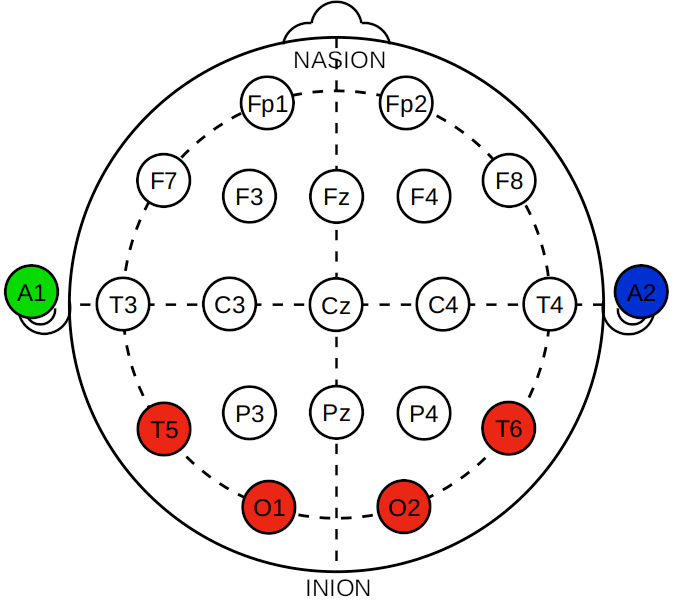
\includegraphics[width=0.5\linewidth]{pictures/Elektroden_Platzierung.jpeg}
%     \caption{10-20 System mit den von uns genutzten Elektroden rot,  Erdungs-Ohrclip grün und \& Referenz-Ohrclip blau gefärbt.}
%     \label{fig:ElektrodenPlatzierung}
% \end{figure}

% \begin{figure}[h!]
%     \centering
%     % TO/DO: Bild mit richtiger Elektrodenplatzierung (Vis. Cortex), Abb. fig:ElektrodenPlatzierung
%     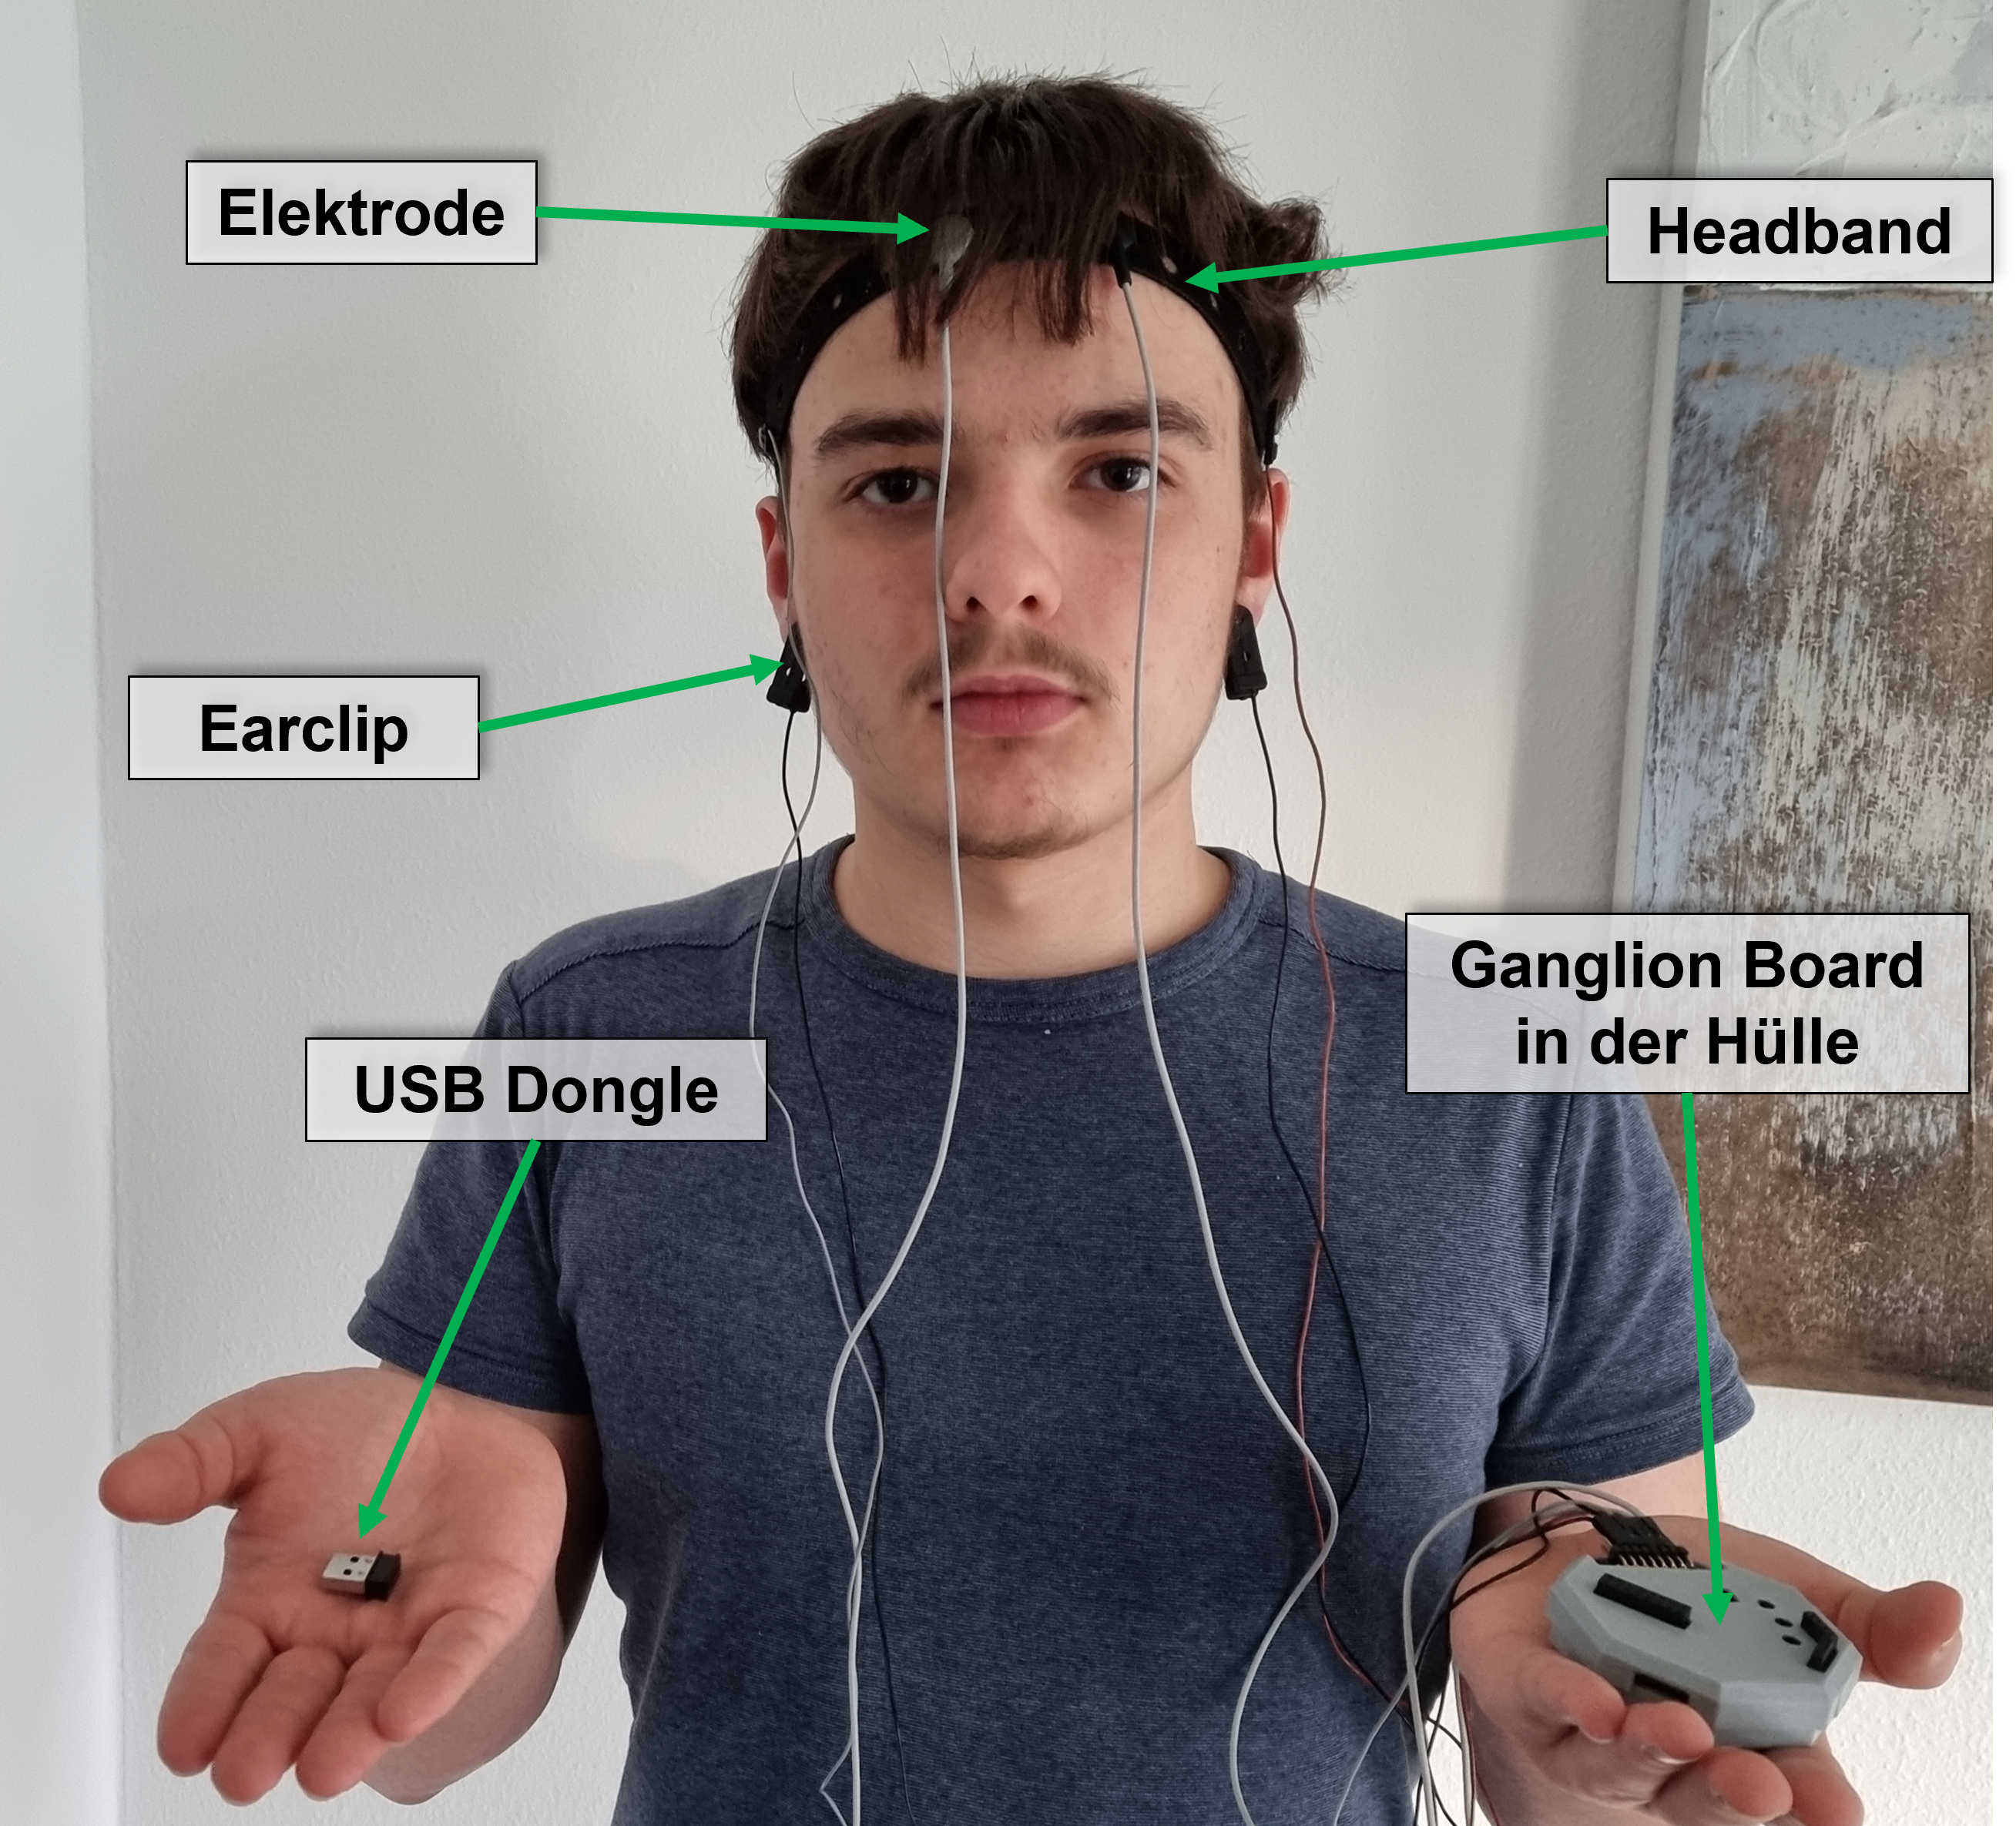
\includegraphics[width=0.46\textwidth]{pictures/EEG-Alex-annotated.png}
%     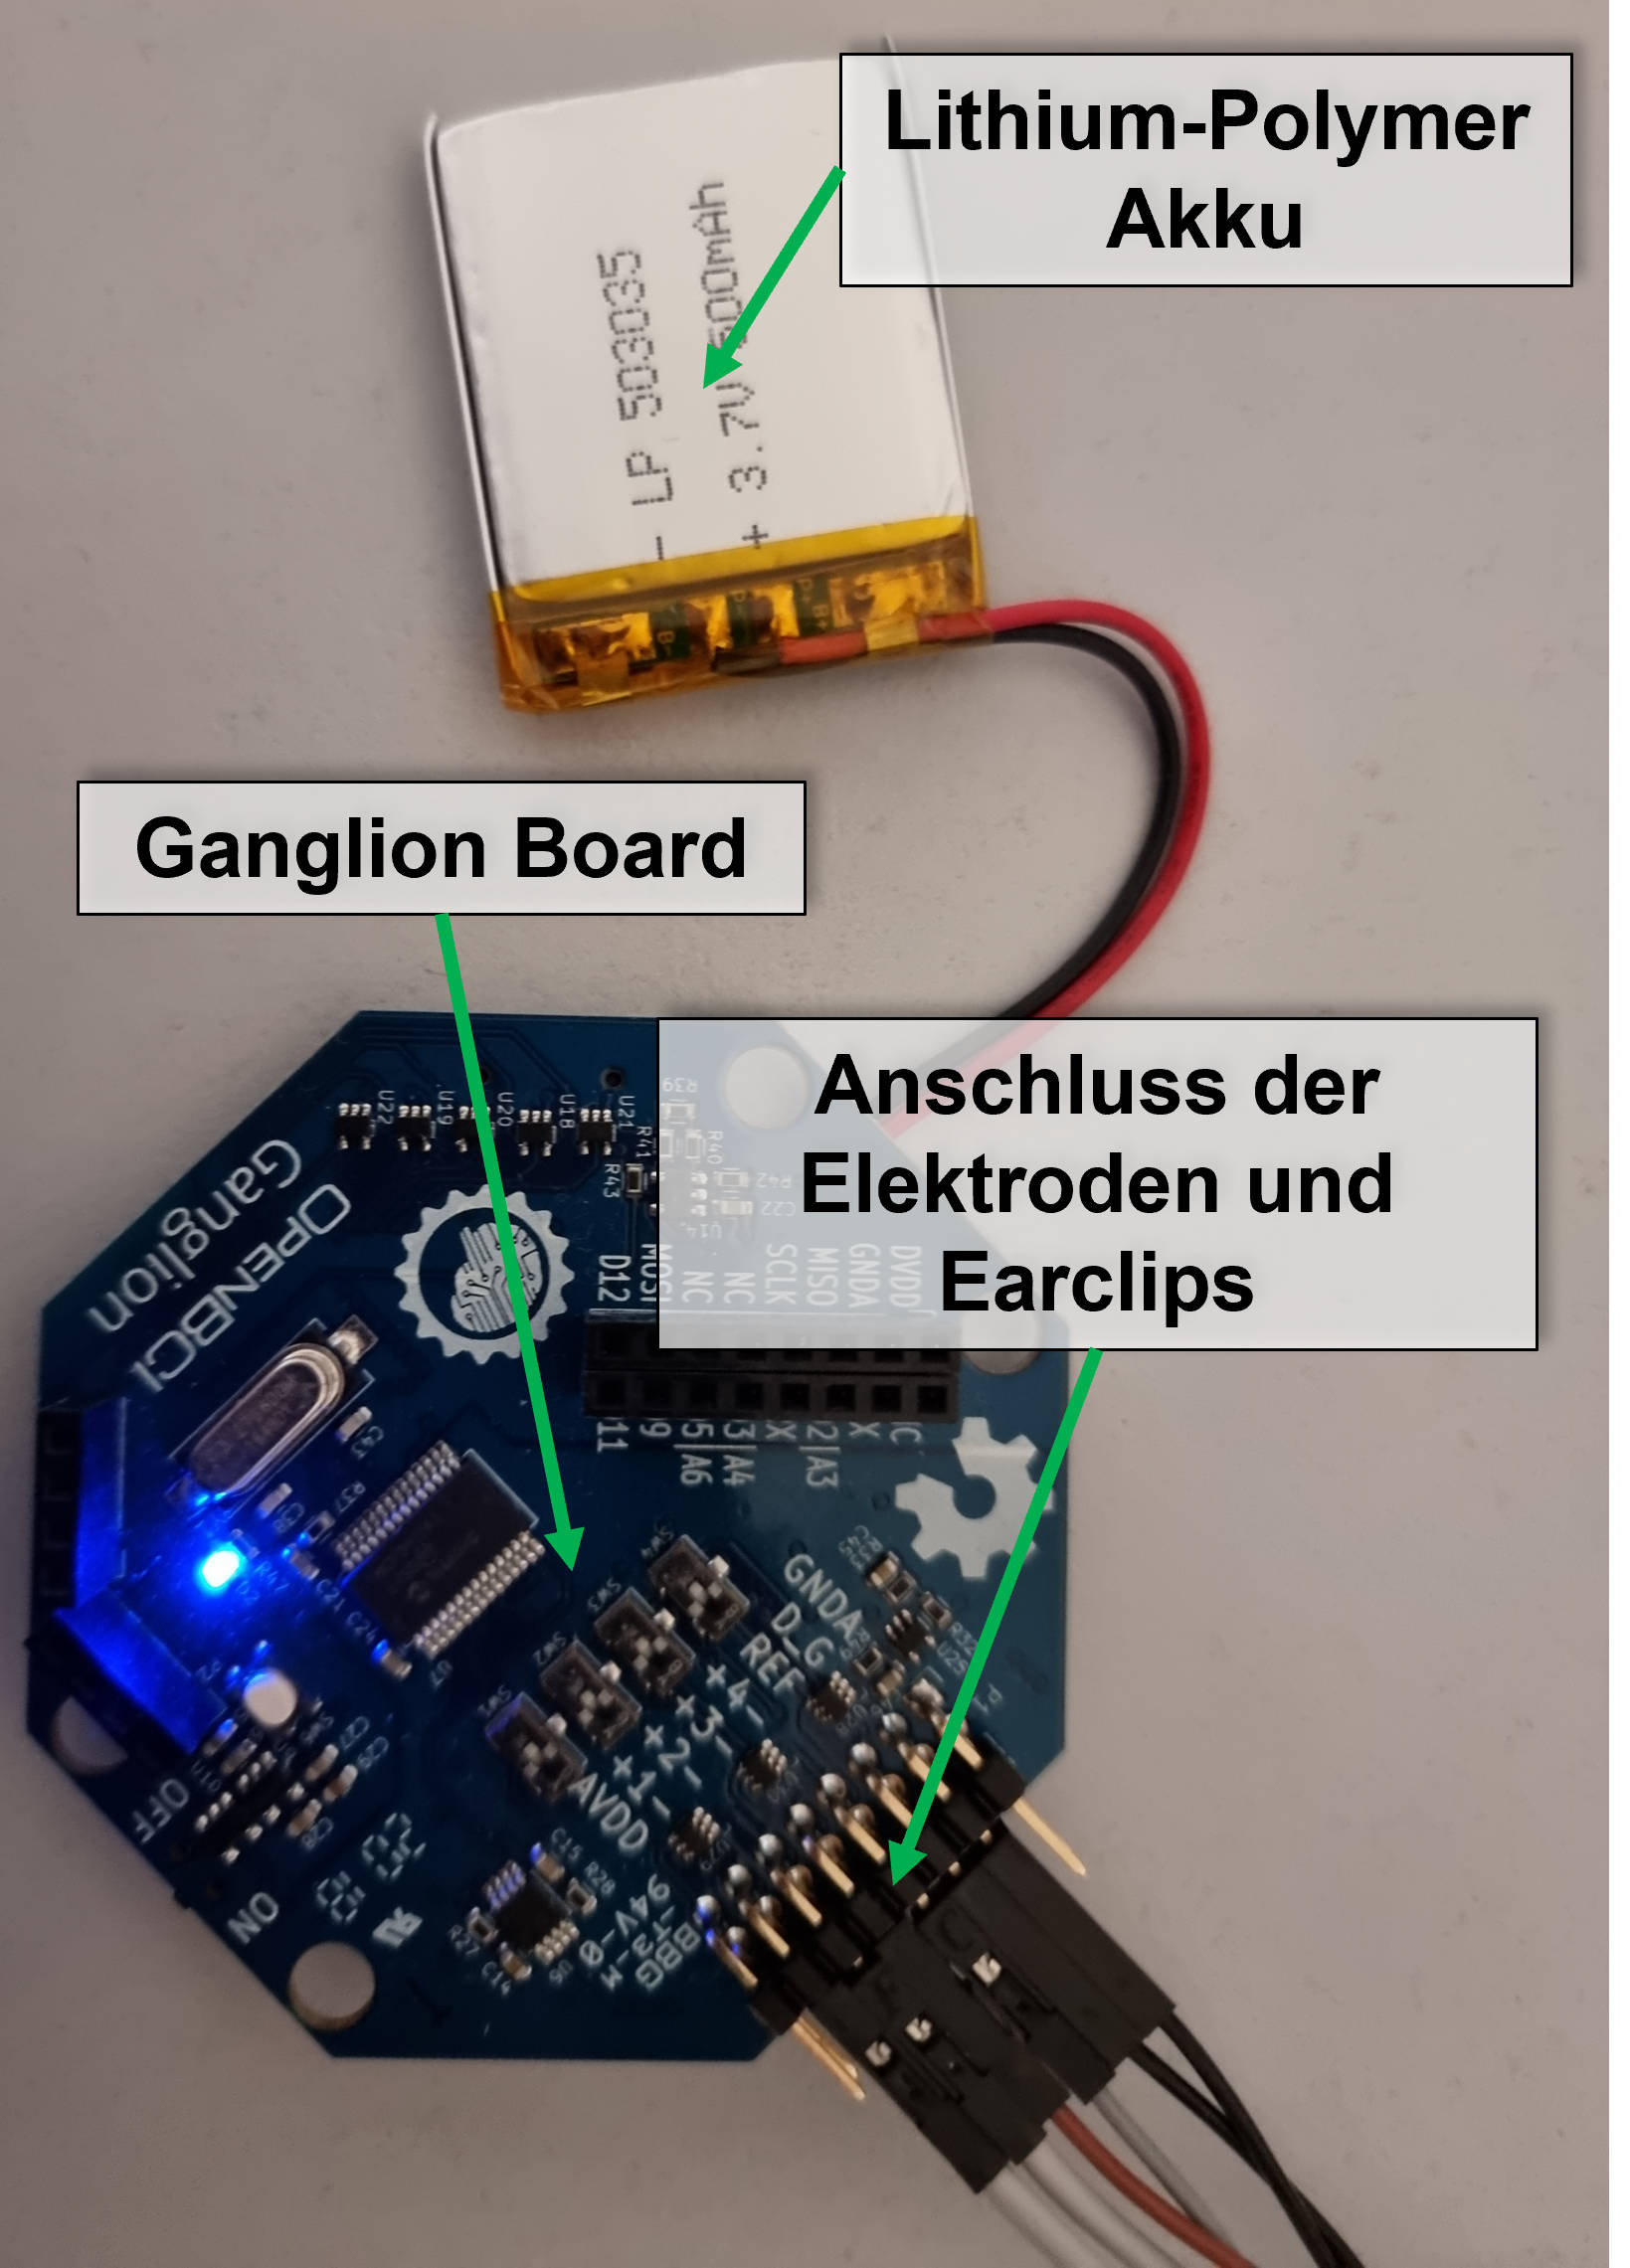
\includegraphics[width=0.3\textwidth]{pictures/Ganglion-Board-annotated.png}
%     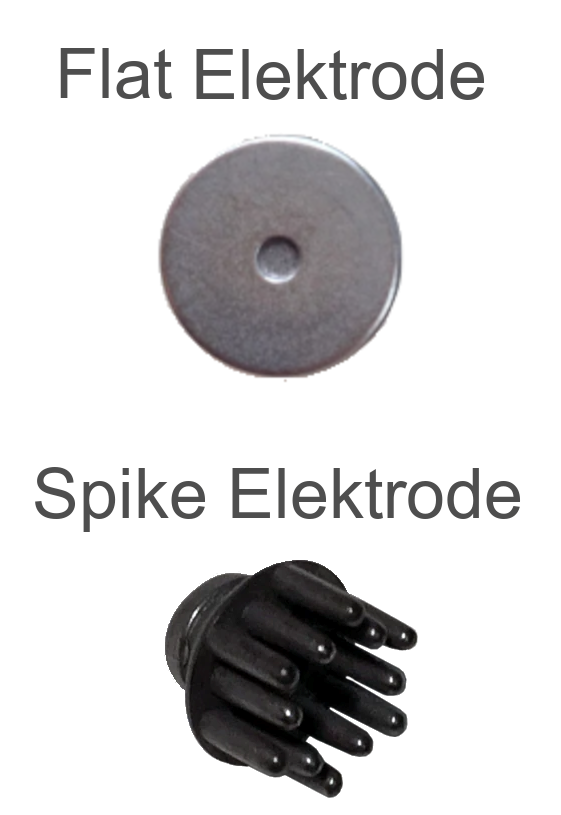
\includegraphics[width=0.15\textwidth]{pictures/spike_flat_elektroden.png}
%     \caption{Das EEG und Zubehör. Links sieht man die typische Anwendung des EEG im Versuchsaufbau. In der Mitte ist das Ganglion Board genauer dargestellt. Rechts sind eine flache Elektrode und eine Spike-Elektrode zu sehen.}
%     \label{EEG-Zubehor}
% \end{figure}

% Als EEG haben wir letztes Jahr das Ganglion Board von OpenBCI verwendet.
% Dieses bietet vier Kanäle, heißt vier Elektroden für die Kopfhaut, sowie eine Referenz- und eine Erdungselektrode. % TODO: Erdungselektrode: Was und wieso?

% Doch obwohl dieses gut funktioniert hat, hat es ein großes Problem: Es kostet ca. \SI{500}{\eur}.
% Dies ist zwar günstig verglichen mit einigen Alternativen, vor allem medizinisch zugelassenen. 
% Für uns ist es jedoch immer noch zu teuer, um unser Ziel zu erfüllen, auch Privatpersonen, vor allem Anfänger, zu interssieren.

% Deswegen wollen wir unser eigenes EEG entwickeln und bauen, mit dem Ziel eine kostengünstigere sowie flexiblere Alternative zu den auf dem Markt angebotenen Modulen qualitativ zu erproben.
% Unser EEG von OpenBCI werden wir also weiter verwenden, sodass wir es mit unserem eigenen EEG vergleichen können. 

% Während wir das EEG entwickelten, wollten wir außerdem bereits mit dem Entiwickeln und Testen einer KI beginnen.
% Dazu haben wir einen Datensatz im Internet gefunden, in welchem der Ersteller mit seinem eigenen 16-Kanal EEG von OpenBCI Daten aufgenommen hat.
% Er hatte das Ziel, 
% Dabei hat er entweder links, rechts oder nicht gedacht und währenddessen EEG-Daten aufgenommen.
% Im folgenden Abschnitt wird nun beschrieben wie wir dabei schrittweise vorgegangen sind.

\subsubsection{Bau unseres eigenen EEG} \label{section:UnserEEG}
 
% Ein EEG stellt vereinfacht nur ein sehr präzises Spannungsmessgerät dar, welches Potentialdifferenzen (Spannungen) im $\mu V$-Bereich messen und anzeigen kann. 
Die Spannungen, die von den Neuronen durch den Schädel dringen, sind zu gering (unterhalb von einigen hundert Mikrovolt), um direkt von einer Messeinheit verarbeitet werden zu können, es muss zunächst eine Verstärkung des aufzuzeichnenden Signals erfolgen. \cite{EEGHausarbeit}
Zweitens müssen die gewünschten Frequenzen vorab mittels aktiver Filter herausgefiltert werden, um unerwünschte Störfrequenzen zu entfernen und so eine genauere Signalanalyse zu ermöglichen.
Je nachdem, welche Phänomene untersucht werden sollen, können unterschiedliche Frequenzbereiche herausgefiltert werden. 
So wären z.B. bei der Analyse von Konzentration oder visueller Verarbeitung vor allem Alpha-Wellen, die in einem Frequenzbereich von 8 bis \SI{13}{\hertz} liegen, relevant. \cite{Praktikum, Birbaumer2010, wiki:Berger-Effekt}
 Drittens wird eine Einheit benötigt, die das Ausgangssignal misst und aufzeichnet, damit es weiterverarbeitet und analysiert werden kann. 
 

 
\begin{figure}[h!]
    \centering
    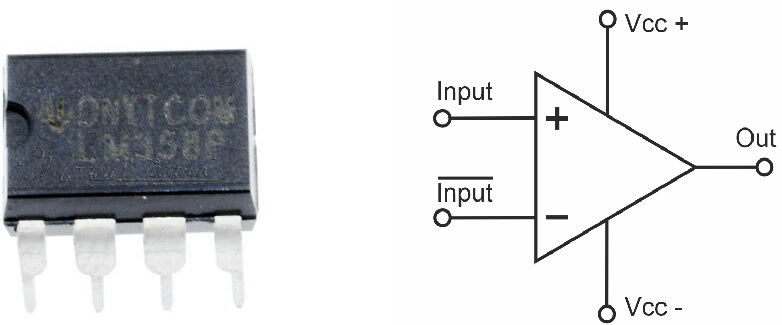
\includegraphics[width=0.6\linewidth]{pictures/OPV.png}
    \caption{Links: 2-fach OPV LM358 in einem DIL-Gehäuse (Dual In-line Package), Rechts: OPV als Schaltbild }
    \label{fig:OPV}
\end{figure}

Sowohl für die Filterung als auch für die Verstärkung werden sogenannte Operationsverstärker (OPV) verwendet. 
In Abb. \ref{fig:OPV} sieht man rechts das Schaltzeichen mit den jeweiligen Anschlüssen und links einen OPV in einem DIL-Gehäuse. 
OPVs finden vor allem in der Mess- und Regeltechnik Anwendung und bestehen aus Transistoren, die zu integrierten Schaltkreisen zusammengefügt werden.
Dabei lässt sich die interne Schaltung eines OPVs allgemein in zwei Schaltungsteile untergliedern, den sogenannten Differenzverstärker, der später für die Potentialmessung wichtig wird, und die dahinter geschaltete Gegentaktendstufe, welche für die Leistungsverstärkung zuständig ist.
Ihr geringer Ausgangswiderstand, der hohe Eingangswiderstand, sowie der hohe Spannungsverstärkungsfaktor machen den OPV passend für die Anwendung als EEG-Verstärker.

OPVs besitzen, neben den Anschlüssen für die Stromversorgung, drei für ihre Funktion wichtige Anschlüsse, einen invertierenden und einen nicht-invertierenden Eingang sowie einen 
Ausgang,  % TODO: Ansteuerung über Ausgang?
über welchen er gesteuert werden kann (Abb. 1 rechts).
Legt man nun bei beiden Eingängen jeweils unterschiedliche Spannungen $U_{1}$ und $U_{2}$ an, so wird am Ausgang des OPVs die Differenz der beiden Spannungen ausgegeben. 
Also gilt: $U = U_{2} - U_{1}$. 
Dies macht man sich nun zu Nutze, um die Spannungen bzw. Potentialdifferenzen zwischen zwei Elektroden zu messen. \cite{Nührmann} 
% Wie oben bereits beschrieben wird dabei immer die Potentialdifferenz zwischen einer Elektrode, die sich auf der Kopfhaut und einer Referenzelektrode, die sich am Ohrläppchen befindent, gemessen. 
Zudem lassen sich mit einem OPV und wenigen weiteren Bauteilen einfach aktive Filter bauen.

Die Grundschaltung für unser EEG beruht auf einem englischsprachigem Internetartikel, in dem eine Verstärkerschaltung für ein EEG beschrieben ist (siehe Abb. 2). \cite{EEGSchaltung} 
%Die von uns angepasste Schaltung ist in Abb. \ref{fig:schaltplan} zu sehen.
Wir mussten die ursprüngliche Schaltung etwas verändern, um den gewünschten Frequenzbereich herauszufiltern.
Basis dieser Schaltung bildet der Instrumentenverstärker AD620AN, welcher extra für EEG- und EKG-Anwendungen entwickelt wurde. 
Ein Instrumentenverstärker ist eine Schaltungskonfiguration aus 3 OPVs, wobei zwei OPVs zu einem Differenzverstärker zusammengeschaltet werden und ein weiterer OPV als Impedanzwandler dahinter geschaltet wird.
Instrumentenverstärker sind sehr präzise und haben einen nochmal höheren Verstärkungsfaktor.
Über Pin 2 und 3 werden die Elektroden angeschlossen, wobei an Pin 2 die Referenzelektrode geklemmt wird. 

\begin{figure}[h!]
    \centering  
    % \newcommand{\twoLabels}[2]{l2 halign=c, l2=#1 and #2}
    \begin{circuitikz}[european, scale=0.5, transform shape]
        \draw (0,0) node[dipchip, num pins=8, no topmark, external pins width=0.0] (C) {AD620};
        % Verbinde Pins 1 und 8 über Widerstand
        \draw 
            (C.pin 1) -- ++ (-0.5,0) 
            to ++(0,1) 
            to [R={\SI{560}{Ω}}, a=$R_g$] ++(2.7,0) 
            to ++(0,-1) 
            to (C.pin 8);
        % Inputs
        \node[left=1.5 of C.pin 2] (inputPos) {};
        \node[left=1.5 of C.pin 3] (inputNeg) {};
        \node[above=0cm of inputNeg, xshift=2em, yshift=-1ex] {\small Input $+$};
        \node[above=0cm of inputPos, xshift=2em, yshift=-1ex] {\small Input $-$};
        \draw
            (C.pin 2) to (inputPos.east)
            (C.pin 3) to (inputNeg.east);
        \draw
            (C.pin 7) to  ++ (1.5,0) to ++ (0,0.75) node[vcc]{\SI{9}{\volt}}
            (C.pin 4) to ++ (-1,0) node[vee]{\SI{-9}{\volt}};
        \node[op amp, right=6 of C, yshift=0.21cm] (opamp1) {OPV1};

        \draw (C.pin 6) to ++(2,0);
        \draw 
            (opamp1.+) node[left] {}
            (opamp1.-) node[left] {}
            (opamp1.out) node[right] {}
            (opamp1.up) -- ++(0,1.5) node[vcc]{\SI{9}{\volt}}
            (opamp1.down) -- ++(0,-1.5) node[vee]{\SI{-9}{\volt}}
            (opamp1.+) to [R=$R_1$,-*, a=\SI{318}{\kohm}] 
            ++(-2,0) to [R=$R_2$,-*, a=\SI{318}{\kohm}] 
            ++(-2,0) to ++(0,-1.5)
            to [C= $C_1$, a={\SI{10}{\nano\farad}}, -*] ++(1.25,0)
            to [C= $C_2$, a={\SI{10}{\nano\farad}}] ++(2.5,0)
            to[short,-*] ++(0,1.5)
            (4.84,-0.3) to (4.84,-4) 
            to [C,l2 halign=c, l2=$C_3$ and {\SI{20}{\nano\farad}}] ++(0,-2) node[rground]{}
            (4.1,-1.8) to (4.1,-2.5) to [R, a2 halign=c, a2=$R_3$ and {\SI{158}{\kohm}}] ++(0,-2) to ++(0,-1.5) node[rground]{} 
            (opamp1.-) to ++(-1,0) to ++(0,1) to ++(3.5,0) to[short,-*] ++(0,-1.5)
            (opamp1.out) to [C= $C_4$,a={\SI{220}{\nano\farad}},-*] ++(2,0) to [C=$C_5$,a={\SI{220}{\nano\farad}}] ++(2,0)
            (11.23,0.25) to [R, l2 halign=c, l2=$R_4$ and {\SI{47}{kΩ}}] ++(0,-4) node[rground]{} 
            (11.23,0.25) to [C, l2 halign=c, l2=$C_6$ and {\SI{220}{\nano\farad}}] ++(0,3) to [short,-*] ++(2,0) to [R, l2 halign=c, a2=$R_5$ and {\SI{220}{kΩ}},-*] ++(0,-3.05);
            %R, l2={A=B} and X, a2={C=D} and Y
        \node[op amp, right=4 of opamp1,yshift=-0.49cm] (opamp2) {OPV2};
        \draw 
            (opamp2.+) node[left] {}
            (opamp2.-) node[left] {}
            (opamp2.out) node[right] {}
            (opamp2.up) -- ++(0,1.5) node[vcc]{\SI{9}{\volt}}
            (opamp2.down) -- ++(0,-1.5) node[vee]{\SI{-9}{\volt}}
            (opamp2.out) to[short,*-] ++(0,3.525) to ++(-2.4,0)
            (opamp2.+) to ++(-0.5,0) to ++(0,-3) node[rground]{}
            (15.6,-0.27) to [R, a=$R_6$, l={\SI{180}{kΩ}},-*] (17.6,-0.27)
            (17.6,-0.27) to[C= $C_7$, a_={\SI{100}{\nano\farad}}] ++(0,-3.5) node[rground]{}
            (17.6,-0.27) to [R, l2 halign=c, l2=$R_7$ and {\SI{180}{kΩ}}] ++(0,3) to[short, -*] ++(1.9,0) to[C=$C_8$, a={\SI{25}{\nano\farad}},-*] ++(0,-2.96);
        \node[op amp, right=4 of opamp2,yshift=-0.45cm] (opamp3) {OPV3};
        \draw 
            (opamp3.+) node[left] {}
            (opamp3.-) node[left] {}
            (opamp3.out) node[right] {}
            (opamp3.up) -- ++(0,1.5) node[vcc]{\SI{9}{\volt}}
            (opamp3.down) -- ++(0,-1.5) node[vee]{\SI{-9}{\volt}}
            (17.6,-0.27) to[R, a=$R_8$, l={\SI{100}{kΩ}}] (opamp3.-)
            (opamp3.+) to ++(-0.5,0) to ++(0,-2.6) node[rground]{}
            (opamp3.out) to [short,*-] ++(0,3.46) to ++(-2.5,0);
        \node[op amp, right=4 of opamp3,yshift=0.48cm] (opamp4) {OPV4};
        \draw 
            (opamp4.+) node[left] {}
            (opamp4.-) node[left] {}
            (opamp4.out) node[right] {}
            (opamp4.up) -- ++(0,1.5) node[vcc]{\SI{9}{\volt}}
            (opamp4.down) -- ++(0,-1.5) node[vee]{\SI{-9}{\volt}}
            (opamp3.out) to [big elko,l=$C_9$, a={\SI{1}{\micro\farad}}] ++(4,0)
            (opamp4.+) to[R,a2 halign=c, a2=$R_{11}$ and {\SI{1}{MΩ}},*-] ++(0,-3.25) node[rground]{}
            (opamp4.-) to[short,-* ] ++(-1.4,0) to ++(-1,0) to [C, l2 halign=c, l2=$C_{10}$ and {\SI{10}{\nano\farad}}] ++(0,3) to [short,-*] ++(1,0) to[R,l2 halign=c, l2=$R_9$ and {\SI{100}{kΩ}}] ++(0,-3)
            (opamp4.out) to ++(0,3.5) to ++(-3.7,0)
            (24.6,0.5) to (24.6,-2.3) to [R,a2 halign=c, a2=$R_{10}$ and {\SI{220}{Ω}}] ++(0,-2)
            (24.6,-4.3) to [vR, l2 halign=c, l2=$R_p$ and \SI{1}{\kohm}, *-] ++(0,-2) node[rground]{}
            (24.6,-4.3) to ++(-0.5,0) to[short,-*] ++(0,-0.74) 
            (opamp4.out) to[big elko, l=$C_{10}$ Output, a={\SI{100}{\micro\farad}},*-] ++(2,0) node[]{};
    \end{circuitikz}
    \caption{Schaltplan des EEG-Verstärkers für eine Elektrode und eine Referenzelektrode, OPV1 bis OPV4 sind alle LM358 (siehe Materialliste)}
    \label{fig:schaltplan}
\end{figure}

Der AD620AN ist ein sehr rauscharmes und leicht zu schaltendes IC, da für die Einstellung des Verstärkungsfaktors nur ein Widerstand nötig ist. Über die Formel im Datenblatt kann man den Verstärkungsfaktor berechnen \cite{AD620AN}:
%
\begin{alignat*}{1}
                & G_1=\frac{\SI{49.4}{\kilo\ohm}}{R_g}+1 
    %\Rightarrow & G_1
    =\frac{\SI{49.4}{kΩ}}{\SI{0.560}{kΩ}}+1 = 89.2 \approx 90 
\end{alignat*}

Hätte man einen größeren Verstärkungsfaktor gewählt, als den der vom Artikel vorgegeben ist, hätte man 
das, dass dabei das Signal noch absolut ungefiltert verstärkt wird, was bedeutet, dass alle Signale bzw. alle Frequenzen, die das eigentlich gewünschte Signal stören oder überlagern, noch mit verstärkt werden. 
Die Filter, die nur eine festgelegte Dämpfung haben, können die Störsignale dann nicht mehr ausreichend unterdrücken. 
Deswegen wird zunächst über den AD620AN nur eine Vorverstärkung vorgenommen. 
Danach findet eine schrittweise Filterung des Signals statt. 
Als allererstes wird über den sog. Notch- oder auch Kerbfilter, der aus OPV1 und vorgeschalteten Widerständen sowie Kondensatoren besteht, das \SI{50}{\hertz}-Netzbrummen herausgefiltert.
Dieses kann das EEG-Signal erheblich stören, da der menschliche Körper unter anderem als eine Art Kondensator fungiert und die \SI{50}{\hertz}-Netzfrequenz des europäischen Stromnetzes zum Eingang des Verstärkers leitet. 

Die Dimensionierung des Verstärkers ist dabei recht einfach. 
Über die gewünschte Grenzfrequenz $f_g = \SI{50}{\hertz}$ sowie die Kapazität der Keramikkondensatoren ($C_1 = C_2 = \SI{10}{\nano\farad}$), siehe Abb.\ref{fig:schaltplan}) lässt sich der Widerstandswert der beiden Widerstände $R_1$ und $R_2$ berechnen.
Dazu wird diese Formel verwendet \cite{Notchfilter,Thomson}: % Ist Grenzfrequenz 50Hz nicht schon gegeben? Wieso dann die Formel? Oder wurde sie umgestellt, um R und C zu bestimmen?
%
\begin{align*}
                &f_g = \frac{1}{R_1 \cdot C_1 \cdot 2 \cdot \pi} \\
\Leftrightarrow &R_1 = \frac{1}{C \cdot 2 \cdot \pi \cdot f_g } = \frac{1}{\SI{10}{\nano\farad} \cdot 2 \cdot \pi \cdot \SI{50}{\hertz}} \approx \SI{318.31}{\kohm}     
\end{align*}
%
Weiterhin gilt für die Schaltung $C_3 = 2 \cdot C_1, R_3 = {R_1} \cdot 0.5$. Es ergibt sich also:
%
\begin{align*}
    C_3 = 2 \cdot \SI{10}{\nano\farad} = \SI{20}{\nano\farad}, \quad
    R_3 = \frac{\SI{318.31}{kΩ}}{2} \approx \SI{159.16}{kΩ} 
\end{align*}
% Wichtig ist hierbei noch zu erwähnen, dass die benötigten Widerstands- und Kapazitätswerte oft keine glatten Zahlen sind. 
Zudem sind die möglichen Widerstandswerte, je nach Baureihe der Komponenten (E12/E24), beschränkt. 
Man muss sich also durch geschickte Reihen- und Parallelschaltung der Widerstände bzw. Kondensatoren den Werten annähern. 
% Die oben angegebenen Werte sind Werte, mit denen wir, für unsere Verhältnisse, möglichst nah an den Sollwert kommen. % TODO: Aber 270 + 33 + 15 = 318 ist doch genau?
Die \SI{318,31}{kΩ}-Widerstände $R_1$ und $R_2$ bestehen z.B. jeweils aus den drei Widerständen \SI{270}{kΩ}, \SI{33}{kΩ} und \SI{15}{kΩ}, was mit einem Gesamtwiderstand von \SI{318}{\kohm} für uns so nah wie möglich am Soll-Wert liegt.
% Das Gleiche gilt auch für den \SI{159}{kΩ}-Widerstand. 

Der OPV2 und die davor geschalteten Komponenten bilden den sog. aktiven Hochpassfilter mit Mehrfachgegenkopplung. 
Dieser Filter arbeitet mit einer Gegenkopplung, was bedeutet, dass das Ausgangssignal über ein passives Filterglied wieder zurück auf den Eingang zurückgeführt wird. 
Dies sorgt für eine bessere Steilheit im Frequenzgang eines Filters. 
Ein Hochpassfilter lässt nur Frequenzen, die oberhalb seiner festgelegten Grenzfrequenz liegen, durch. 
Der Frequenzgang beschreibt den Frequenzverlauf in Abhängigkeit zur Dämpfung und wird in einen Sperr- und einen Durchlassbereich sowie einen dazwischenliegenden Übergang gegliedert. 
Der ideale Filter würde bei der Grenzfrequenz eine unendliche Dämpfung erreichen. 
In der Realität verläuft der Übergang vom Durchlass- in den Sperrbereich nicht abrupt, sondern, wenn eine logarithmische Skalierung verwendet wurde, linear.
In Abb. \ref{fig:LHP} kann man dies gut sehen.

\begin{figure}[h!]
    \centering
    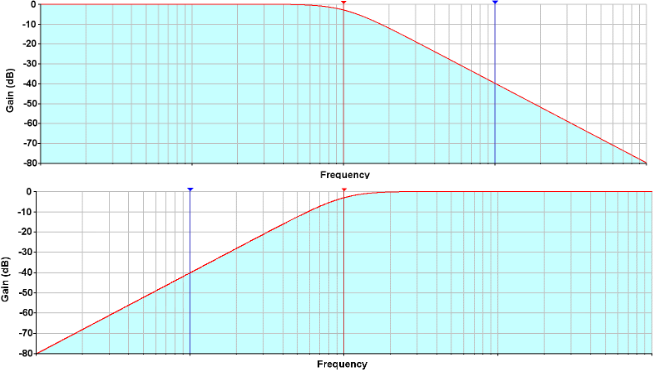
\includegraphics[scale=0.5]{pictures/Low_Highpass.png}
    \caption{Typischer Frequenzgang eines Tiefpassfilters (oben) und Hochpassfilters (unten), Rote Linie ist die Grenzfrequenz, Blaue Linie eine Dekade Abstand zur Grenzfrequenz, um Steilheit zu bestimmen}
    \label{fig:LHP}
\end{figure}

Die Steilheit beschreibt die Steigung dieser Übergangsgerade und wird in \si{\dB\per\dek} angegeben. 
Eine Dekade beschreibt den Abstand zwischen $10^x$\si{\hertz} und $10^{x+1}$\si{\hertz}. 
Also z.B den Abstand zwischen \SI{10}{\hertz} und \SI{100}{\hertz} oder \SI{1000}{\hertz} und \SI{10000}{\hertz}. 
Je steiler die Übergangsgerade, desto besser ist der Filter. 
Des Weiteren ist an der Grenzfrequenz immer ein Abfall von ca. \SI{6}{\dB} zu beobachten, wenn eine Mehrfachrückkopplung verwendet wird. 
Bei aktiven Filtern, wie sie hier beschrieben sind, erreicht man eine Steilheit von \SI{40}{\dB\per\dek}. 
Für die Berechnung der Grenzfrequenz des Hochpasses mit Mehrfachgegenkopplung benötigen wir eine etwas andere Formel, als die, die wir beim Notchfilter verwendet haben. Da alle Werte gegeben sind wird die Berechnung nur bestätigt:
% Für eine genaue Herleitung möchten wir auf \cite{aktivHochpass} verweisen, da die Herleitung den Rahmen der Arbeit sprengen würde. % TODO: Wenn nicht selbst hergeleitet, müsste es sowieso nicht in der Arbeit stehen
%
\begin{align*}
                & f_g=\frac{1}{2 \cdot \pi \cdot C_5 \cdot \sqrt{{R_4} \cdot R_5}} 
    \Rightarrow & f_g =\frac{1}{2 \cdot \pi \cdot \SI{220}{\nano\farad} \cdot \sqrt{\SI{47}{\kohm} \cdot \SI{220}{\kohm}}} = \SI{7.114}{\hertz} 
    \approx \SI{7}{\hertz}
\end{align*}
  
Der Hochpass hier ist auf eine Grenzfrequenz von ca. \SI{7}{\hertz} eingestellt. 
Im Anschluss auf den Hochpass folgt ein Tiefpass (OPV3), der die selbe Funktionsweise hat, mit der Ausnahme, dass er nur die Frequenzen \textbf{unter} der Grenzfrequenz durchlässt.
Mit der Formel zur Berechnung der Grenzfrequenz eines Tiefpasses ergibt sich für uns \cite{aktivHochpass}:
%
\begin{align*}
            & f_g = \frac{1}{2 \cdot \pi \cdot \sqrt{R_7 \cdot R_8 \cdot C_7 \cdot C_8}}
\Rightarrow & f_g=\frac{1}{2 \cdot \pi \cdot \sqrt{\SI{180}{\kohm} \cdot \SI{100}{\kohm} \cdot \SI{100}{\nano\farad} \cdot \SI{25}{\nano\farad} } } = \SI{23.72}{\hertz} \approx \SI{24}{\hertz}
\end{align*}
 
Der Tiefpass ist in unserem Fall für eine Grenzfrequenz von \SI{24}{\hertz} eingestellt.  

\newcommand{\RPot}{R_{\textrm{Pot}}}
Nach einem RC-Filterglied folgt dann der Endverstärker, welchen OPV4 mit entsprechenden Zusatzkomponenten bildet. 
Hierbei handelt es sich um einen nicht-invertierenden Verstärker, dessen Verstärkung über den Spannungsteiler, der aus dem \SI{100}{\kohm}-Widerstand, dem \SI{220}{\kohm}-Widerstand und dem \SI{1}{\kohm}-Potentiometer $R_{\textrm{Pot}}$ besteht, eingestellt werden kann.
Mit der folgenden Formel lässt sich die minimale ($R_p = \SI{1}{\kohm}$) und maximale ($R_p = \SI{0}{\ohm}$) Verstärkung berechnen \cite{EEGSchaltung}:
%
\begin{align*}
   & G_2=\frac{R_9}{R_{10}+R_p}+1 \\ % TODO: Einheit von 1?
    \xRightarrow{R_p = \SI{0}{\kohm}} & G_2=\frac{\SI{100}{kΩ}}{\SI{0.22}{kΩ}+\SI{0}{Ω}}+1= 455 \\
    \xRightarrow{R_p = \SI{1}{\kohm}} & G_2=\frac{\SI{100}{kΩ}}{\SI{0.22}{kΩ}+\SI{1}{kΩ}}+1= 83
\end{align*}

Insgesamt ergibt sich bei unserem EEG also ein Verstärkung von maximal $G_1 * G_2  \Rightarrow 455 \cdot 90 = 40950$.
Der Verstärker wurde bereits mittels Oszilloskop getestet, dabei fiel auf, dass das Signal noch durch \SI{50}{\hertz}-Brummen gestört wird.
Deswegen wird das ganze EEG nun über \SI{9}{\volt}-Blockbatterien betrieben, um dem \SI{50}{\hertz}-Brummen eines Netzteils entgegenzuwirken, und zusätzlich noch über einen Masseanschluss geerdet. Alle diese Dinge hatten ein positiven Einfluss auf das EEG-Signal, reichten aber immer noch nicht ganz aus, um gute Ergebnisse zu erzielen.
Deswegen ziehen wir in Erwägung, am Ende der Schaltung noch einen weiteren Notchfilter zu schalten. 
Der ganze Aufbau ist provisorisch auf einem Steckbrett erfolgt (s. Abb. \ref{fig:Schaltung}), soll aber fest auf einer Platine verlötet und in ein Gehäuse verbaut werden, sobald es ausreichend getestet wurde und zufriedenstellende Ergebnisse geliefert hat.
 \begin{figure}[h!]
    \centering
    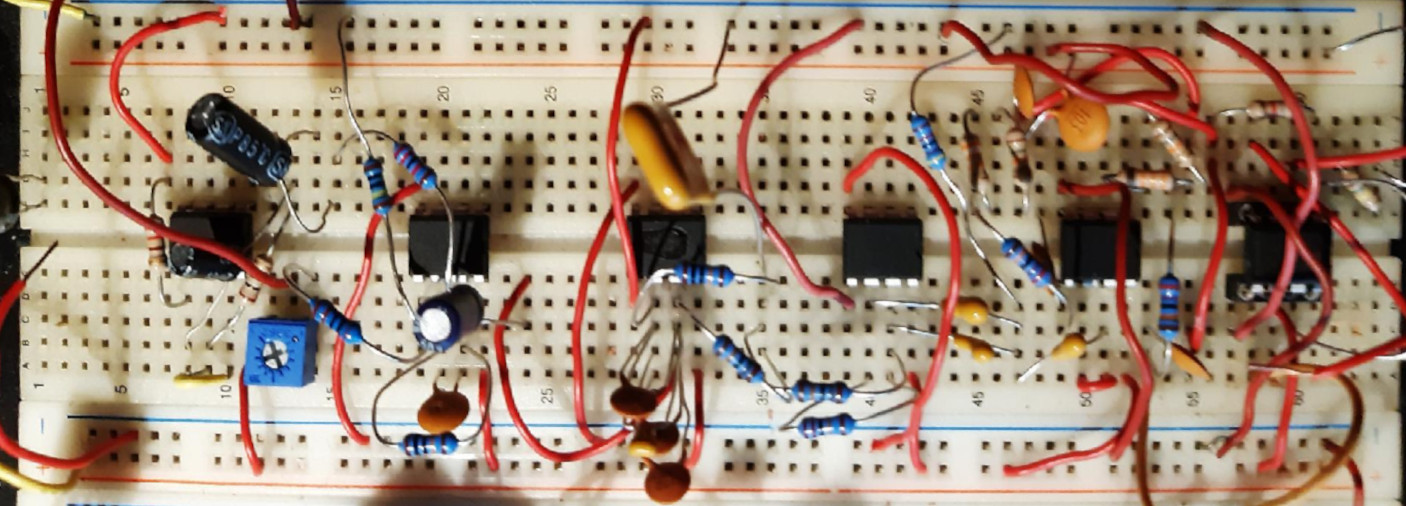
\includegraphics[width=0.5\linewidth]{pictures/Schaltung_cropped.jpeg}
    \caption{Schaltung fertig auf einem Steckbrett aufgebaut}
    \label{fig:Schaltung}
\end{figure}
Unabhängig davon haben wir parallel an einer Mess- und Ausleseeinheit gearbeitet, die ein wichtiger Teil für weitere Datenverarbeitung darstellt. 
Diese Einheit besteht aus dem Analog/-Digitalwandler (ADC) MCP3208, der an an die SPI-Schnittstelle eines Raspberry Pi 3B angeschlossen wird.
Der MCP3208 besitzt 8 Analoge Eingänge und hat eine Auflösung von 12 Bit sowie eine Abtastrate von 100ksp/s. \cite{ADC}

% Dies sind wichtige Daten, da über die Auflösung die Messgenauigkeit festgelegt wird. 
Ein ADC funktioniert, indem er einen Spannungsmessbereich, der über einen Referenzpin am IC festgelegt wird, in einzelne digitale Zustände aufteilt. 
Über die Auflösung kann berechnet werden, in wie viele Zustände der ADC den Messbereich unterteilt, bei 12 Bit ergeben sich $2^{12}=4096$ Zustände. 
Das bedeutet, dass bei einer Referenzspannung $U_\textrm{Ref}$ von \SI{5}{\volt} die Eingangsspannungen in 4096 Zustände unterteilt werden, sodass das kleinste erkennbare Spannungsintervall $U_\textrm{Intervall} = \frac{\SI{5}{\volt}}{4096} \approx \SI{1.2}{\milli\volt}$.
Der ADC schreibt also allen Vielfachen von \SI{1.2}{\milli\volt} eine digitale Ganzzahl zu. 
So entsprächen \SI{2.4}{\milli\volt} dem Wert 2, \SI{3.6}{\milli\volt} dem Wert 3, usw. 
Nun lässt sich aus dem Digitalwert, den uns der MCP3208 liefert, ein Spannungswert berechnen:
%
\[
    U = U_\textrm{Intervall} \cdot \textrm{Digitalwert}
\]

% Eine höhere Messgenauigkeit des EEGs kann sowohl durch eine höhere Auflösung als auch durch eine kleinere Referenzspannung erreicht werden. 
Die Messgenauigkeit ist in diesem Fall mehr als ausreichend, da durch den EEG-Verstärker bei maximaler Verstärkung die untere Grenzspannung für EEG-Messungen von \SI{1}{\micro\volt} auf ca. \SI{41}{\milli\volt} verstärkt wird. 

Ein Programm, um den Analog/-Digitalwandler auszulesen, wurde bereits geschrieben. 
Der Zusammenbau beider Komponenten steht jedoch noch aus, da sowohl der EEG-Verstärker als auch die Ausleseeinheit noch verbessert und ausreichend getestet werden müssen. 
 
 
\subsection{Fourier-Analyse}

Die Fourier-Analyse kann die verschiedenen zugrundeliegenden Frequenzen von Datenfolgen oder Funktionen bestimmen, indem diese in Sinus-Kurven mit verschiedenen Frequenzen zerlegt werden, welche summiert dem ursprünglichem Signal entsprechen.
Zu diesem Zweck wird jeder Frequenz eine Amplitude zugeordnet.
Die Fourier-Analyse dient also zur Spektralanalyse.

Wir nutzen in unserem Projekt die Fast Fourier Transformation (FFT), welche lediglich eine komplexere aber effizientere Form der Diskreten Fourier Transformation (DFT) ist.
% TODO: Beschreibung DFT?
Aus der FFT folgt ein Array (eine Liste) an komplexen Zahlen. 
Der Index eines Wertes in der Liste bestimmt die Frequenz dieses Wertes
(erster Wert: 1 Hertz, zweiter Wert: 2 Hertz, etc.). Nun muss für jede komplexe Zahl der Abstand zum Ursprung bestimmt werden, also der absolute Betrag. 
Dieser entspricht dann der Amplitude des Signals bei dieser Frequenz. So lässt sich bestimmen, welche Frequenzen am stärksten im Signal vorkommen. Außerdem können auf diese Weise Frequenzen herausgefiltert werden, indem die Werte bei den entsprechenden Indices auf 0 gesetzt werden. 

Eine Spektralanalyse ergibt v.a. bei EEG-Daten Sinn, da diese inherent auf Frequenzen aufgebaut sind, denn viele Neuronen im Gehirn, v.a. mit ähnlichen Aufgaben, sind synchronisiert, sodass sie eine ähnliche Frequenz haben.
Es lassen sich verschiedenen Aktivitätsstufen der Neuronen und Aufgaben-/Gehirnbereichen verschiedene Frequenzbereiche zuweisen, wie schon in \nameref{section:UnserEEG} beschrieben.

Eine FFT kann Elektroenzephalogramme verlustfrei repräsentieren.
Dies lässt sich erkennen, indem man mithilfe der durch die FFT entstandenen Spektralanalyse die Daten rekonstruiert (Inverse Fast Fourier Transformation, IFFT). 
Es werden dazu die Sinus-Kurven der Frequenzen mit den entsprechenden Amplituden multipliziert und dann addiert.
Wie in Abb. \ref{fig:ifft} sichtbar, ist diese Rekonstruktion nicht von den originalen Daten unterscheidbar. % TODO: Gesamtdifferent oder anderes mathematische Maß für Ähnlichkeit anstelle / zusätzlich zu graphischem?

\begin{figure}[h!]
    \centering
    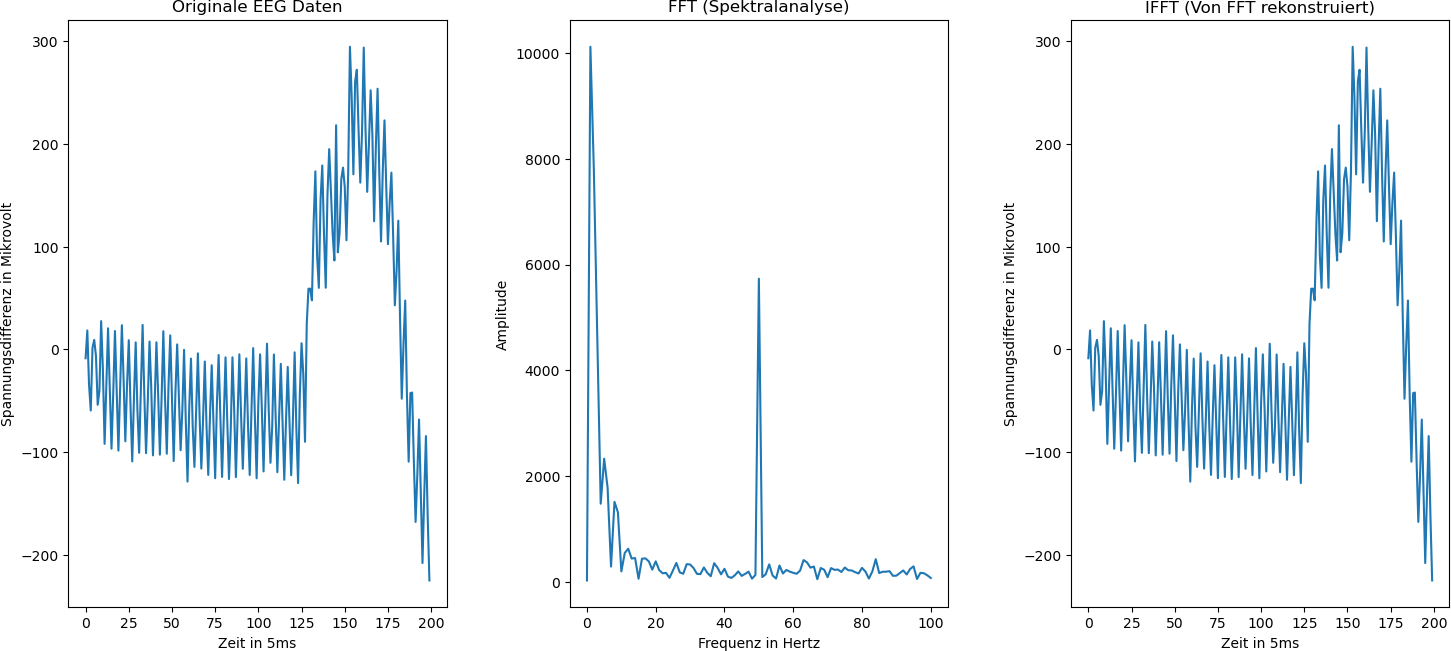
\includegraphics[width=0.8\linewidth]{pictures/blink_fft_ifft_cropped.png}
    \caption{Links: Originale EEG Daten, Mitte: Die Amplituden der Frequenzen dieser Daten, Rechts: Die Umkehrung der Frequenzdaten. Da der rechte Graph dem linken sehr ähnlich ist, lässt sich erkennen, dass es bei der Fourier Analyse keinen großen Informationsverlust gibt.}
    \label{fig:ifft}
\end{figure}

\subsection{Neuronales Netz}

Ein neuronales Netzwerk besteht aus drei Teilen: der Eingabeschicht, den verdeckten Schichten und der Ausgabeschicht. 
Die Eingabeschicht ist eine Liste aus Zahlen. 
Sie gibt an, welche Eingaben das Netzwerk bekommen soll, z.B. die Helligkeit der Pixel eines Graustufen-Bildes.
Die verdeckten Schichten sind eine Ansammlung von in mehrere Schichten unterteilten Neuronen.

Jedes Neuron besitzt eine sogenannte Aktivierung, die meist als Zahl im Intervall zwischen 0 und 1 oder zwischen  -1 und 1 angegeben werden kann. 
Die Neuronen verschiedener Schichten sind durch sogenannte Gewichte (\eng{weights}) verbunden, die ebenfalls einen beliebigen Wert haben können.
Die Ausgaben / Vorhersagen des neuronalen Netzwerkes werden von den Aktivierungen der Neuronen in der Ausgabeschicht abgelesen.

\subsubsection{Forward Pass}
Bei neuronalen Netzwerken gibt es zwei wichtige Verfahren: Den Forward Pass und die Backpropagation.
Ersteres beschreibt das Weiterreichen % TODO: Formulierung?
von Eingabewerten durch das Netzwerk.
Zuerst werden die Aktivierungen der Neuronen in der Eingabeschicht gesetzt und danach mithilfe der verbindenden Gewichte zuerst die Netzeingaben und dann die Aktivierungen der Neuronen der nächsten Schicht berechnet, welche dann wiederum für die nächsten Schicht verwendet werden und so weiter.
Dadurch werden die Eingaben von Schicht zu Schicht bis zur Ausgabe weiterverarbeitet.
Das konkrete Verfahren zur Berechnung der Netzeingabe ist abhängig von Art der Schicht.
%Die Netzeingabe, die aus den Aktivierungen der vorherigen Schicht berechnet wird, kann direkt als Aktivierung eines Neurons verwendet werden.

Man wendet auf diese Netzeingabe eine Aktivierungsfunktion an, um die Aktivierung zu erhalten.
Dies sorgt dafür, dass es keine Linearität zwischen Eingaben und Ausgaben gibt, wodurch das Netzwerk auch nichtlineare Zusammenhänge modellieren kann. % TODO: Quelle

\begin{figure}[h!]
    \centering
    \begin{tikzpicture}
    \begin{axis}[height=4.5cm, width=15cm,
        xlabel={Netzeingabe}, ylabel={Aktivierung}, domain={-10:10}, samples=100,
        ymax=1.5, no markers, legend pos=south east, every plot/.style = {line width = 2pt}, font=\small]
        \addplot+[line width = 1.2pt] {1 / (1 + 2.71828^(-x))};
        \addplot+[line width = 1.2pt] {tanh(x)};
        \addplot+[line width = 1.2pt, green!50!black] {(x>=0)*x};
        \legend{$\sig(x)$, $\tanh(x)$, ReLU};
    \end{axis}
    \end{tikzpicture}
    \caption{Aktivierungsfunktionen im Vergleich}
    \label{fig:act_funcs}
\end{figure}

Letztes Jahr haben wir dafür die Sigmoid-Funktion genutzt, welche die Aktivierung auf Werte zwischen 0 und 1 beschränkt (s. Abb. \ref{fig:act_funcs}).
%
\[
    \sig(x) = \frac{1}{1+e^{-x}}
\]

Doch dieses Jahr setzen wir auf die $\tanh$-Aktivierungsfunktion (Hyperbeltangens) \cite{wiki:Hyperbeltangens}, bei der die Ausgabe immer zwischen -1 und 1 liegt (s. Abb. \ref{fig:act_funcs}), da sie 
eine bessere Lernleistung für neuronale Netze bietet. \cite{blog:activationFunctions, blog:tanhVsSigmoid} 
%
\[
    \tanh(x) = 1-\frac{2}{\mathrm{e}^{2x}+1}
\]

Außerdem nutzen wir die ReLU-Aktivierungsfunktion, da sie besonders gut für die Convolutional Schichten geeignet ist. Die ReLU-Aktivierungsfunktion gibt für alle negativen Eingabewerte 0 aus und lässt alle positiven Eingabewerte unverändert.

\subsubsection{Backpropagation}



%indem die Differenz zwischen der tatsächlichen Aktivierung nach dem Forward Pass und den zugewiesenen korrekten Ausgaben gebildet wird.

% \begin{figure}
%     \centering
%     \begin{tikzpicture}
%         \node (forward1) {Forward Pass};
%         \node[left=1cm of forward1] (train_inputs) {Trainingsdaten: Eingaben};
        
%         \node[below=1cm of forward1] (backprop) {Backpropagation};
%         \node[below=1cm of train_inputs] (train_outputs) {Trainingsdaten: Ausgaben};

%         \draw
%             (train_inputs) edge[->] (forward1)
%             (forward1) edge[->] (backprop)
%             (train_outputs) edge[->] (backprop);
        
%         \node[below=1cm of backprop] (forward2) {Forward Pass};
%         \node[below=1cm of train_outputs] (test_inputs) {Testdaten: Eingaben};
%         \draw
%             (backprop) edge[->] (forward2) node[midway, left] {verbessert}
%             (test_inputs) edge[->] (forward2);
        
%         \node[below=1cm of forward2] (round) {Ausgaben runden};
%         \node[below=1cm of test_inputs] (test_outputs) {Testdaten: Ausgaben};
%         \draw[->] (forward2) -- (round);
%         \draw (test_outputs) -- (round) node[midway] (mid) {};
%         \node[below=1cm of mid] (test_acc) {Testdatengenauigkeit};
%         \draw[->] (mid) -- (test_acc) node[midway, left] {vergleichen};
%     \end{tikzpicture}
%     \caption{Supervised Learning}
%     \label{fig:supervised_learning}
% \end{figure}

% TODO: Different passend?

\newcommand{\textD}{$\delta$}

Der Forward Pass bildet den ersten Schritt der Backpropagation, die für das Lernen des Netzwerkes verantwortlich ist. Dabei werden, nachdem alle Aktivierungen gesetzt wurden, die Aktivierung der letzten Schicht, also die Ausgaben, bewertet.
Da wir Supervised Learning verwenden, benötigen wir dafür Trainingsdaten, denen wir vorher die korrekten Ausgabedaten zugewiesen haben.
Mit diesen wird dann jedes einzelne Ausgabeneuron mit einer sogenannten Verlustfunktion "bewertet". Je weiter die Ausgaben des neuronalen Netzwerks von dem Ideal (im Trainingsdatensatz vorgegebene Ausgabedaten) abweichen, desto höher der sogenannte Verlust, der mit der Verlustfunktion berechnet wird.

Diese Differenz zwischen ist-Zustand und soll-Zustand wird nun in der Backpropagation verwendet, um die Gewichte anzupassen, denn mit ihr kann der sogenannte \textD-Wert der Ausgabeschicht bestimmt werden.
Dieser entspricht der Änderung der Aktivierung eines Neurons, die notwendig wäre, damit ein Forward Pass ein besseres Ergebnis.

Um diese \textD-Werte für die Neuronen der verdeckten Schichten zu berechnen, werden natürlich die \textD-Werte der dahinter liegenden Schichten benötigt, da die benötigte Änderung nur von den Ausgaben aus bestimmt werden kann.
Aufgrund dieses Zurückpropagierens der \textD-Werte zur Eingabeschicht hin kommt auch der Name Backpropagation.
Auf die Berechnung des \textD-Werts werden wir dieses Jahr nicht weiter eingehen, da sie für uns nicht direkt relevant ist und wir für unsere neuronale Netzwerke das Julia-Package Flux einsetzen, welches diese Arbeit übernimmt.

Mithilfe dieses \textD-Werts wird dann bestimmt, wie die Gewichte des Netzwerks angepasst werden müssten, um diese gewünschte Änderung umzusetzen:
%
\form{\[
	\Delta W_{i,j} = \eta * \delta_i * a_j
\]}

\noindent wobei $i$ das Neuron näher zur Ausgabe, $j$ das Neuron näher zur Eingabe und $W_{i,j}$ das Gewicht zwischen diesen beiden ist.

Die Multiplikation mit $a_j$ findet statt, um zu ermöglichen, dass die Änderung der Gewichte entsprechend ihres tatsächlichen Einflusses geschieht. Das bedeutet, wenn ein Gewicht mit einem Neuron verbunden ist, welches kaum aktiv ist (eine niedrige Aktivierung hat), wird das Gewicht zu diesem auch kaum angepasst.

$\eta$ ist die sogenannte Lernrate.
Sie ist meist ein sehr niedriger Wert (0.01, 0.0001, etc.) und ist wichtig für das Kernkonzept des Lernen eines neuronalen Netzwerks:
Sie sorgt dafür, dass bei jedem Trainingsdatensatz die Gewicht nur etwas an diesen angepasst werden, sodass das gesamte Training die Gewichtsanpassungen aller Trainingsdatensätze und somit hoffentlich auch eine Generalisierung dieser darstellt.
Umgesetzt wird diese Änderung einfach mit
\form{\[
    W_{i,j} = W_{i,j} + \Delta W_{i,j}
\]}

\subsubsection{Verlustfunktion}

Insgesamt lässt sich sagen, dass ein neuronales Netzwerk versucht, die Verlustfunktion zu minimieren.
Es gibt viele verschiedene Arten von Verlustfunktionen %, die alle auch verschiedene Vor- und Nachteile haben.
und wir haben uns dazu entschieden, den Mean Squared Error (kurz MSE) als Verlustfunktion zu nutzen, welcher sich mit folgender Formel berechnen läßt:
%
\form{ \[
	C_0 = (a_0 - y)^2
\]}
\noindent wobei $C_0$ der Verlust der Ausgabeschicht (Schicht $0$, da Indexierung der Schichten bei der Ausgabe beginnt), $a_0$ der Vektor aller Aktivierungen der Ausgabeschicht, und $y$ ein Vektor der richtigen Ausgaben für die Eingaben, mit denen die Aktivierungen berechnet wurden, ist.

\subsubsection{Fully Connected Schichten} 

Bei Fully Connected Schichten sind alle Neuronen eines Layers mit allen Neuronen des nächsten Layers verbunden, außerdem hat typischerweise jedes Neuron einen sogenannten Bias, der hinzu addiert wird (s. Abb. \ref{fig:dense_nn}).

\begin{figure}[h!]
    \def\layersep{6cm}
    \def\biasDist{0.6}
    \centering
    \adjustbox{scale=0.8}{%
    \begin{tikzpicture}[
        % scale=1.2,
        shorten >=1pt,->,draw=black!70, node distance=\layersep,
        neuron/.style={circle,fill=black!25,minimum size=20,inner sep=0},
        edge/.style 2 args={pos={(mod(#1+#2,2)+1)*0.33}, font=\tiny},
        distro/.style 2 args={
            edge={#1}{#2}, node contents={}, minimum size=0.6cm, path picture={\draw[double=orange,white,thick,double distance=1pt,shorten >=0pt] plot[variable=\t,domain=-1:1,samples=51] ({\t},{0.2*exp(-100*(\t-0.05*(#1-1))^2 - 3*\t*#2))});}
          },
        weight/.style 2 args={
            edge={#1}{#2}, node contents={\pgfmathparse{0.35*#1-#2*0.15}\pgfmathprintnumber[fixed]{\pgfmathresult}}, fill=white, inner sep=2pt
          }
      ]
    % Input layer
    \foreach \y in {1,...,2}
        \node[neuron, fill=green!40] (i\y) at (0,\y+1) {$i_\y$};
    \node[neuron, fill=orange!40, above=\biasDist of i2] (b1) {$b_1$};
    % Hidden layer
    \foreach \y in {1,...,4}
        \path node[neuron, fill=blue!40] (h\y) at (\layersep,\y) {$h_\y$};
    \node[neuron, fill=orange!40, above=\biasDist of h4] (b2) {$b_2$};
    % Output node
    \node[neuron, fill=red!40] (o) at (2*\layersep,2.5) {$O$};
    
    % Connect every node in the input layer with every node in the hidden layer.
    \foreach \source in {1,...,2}
        \foreach \dest in {1,...,4}
            \path (i\source) edge (h\dest);
    % Connect bias in the input layer with every node in the hidden layer.
    \foreach \dest in {1,...,4}
        \path[red!20] (b1) edge (h\dest);
    % Connect every node in the hidden layer with the output layer
    \foreach \source in {1,...,4}
        \path (h\source) edge (o);
    % Connect bias in the hidden layer with the output layer
    \path[red!20] (b2) edge (o);
        
    % Draw weights for all regular edges.
    \foreach \i in {1,...,2}
        \foreach \j in {1,...,4}
            \path (i\i) -- (h\j) node[weight={\i}{\j}];
    \foreach \i in {1,...,4}
        \path (h\i) -- (o) node[weight={\i}{1}];
    % Draw weights for bias edges.
    \foreach \j in {1,...,4}
        \path (b1) -- (h\j) node[weight={3}{\j}];
    \path (b2) -- (o) node[weight={5}{1}];
    \end{tikzpicture}
    }
    \caption{Ein Beispiel für ein neuronales Netzwerk bestehend aus einer Eingabeschicht($i_1$ und $i_2$) und zwei Fully Connected Schichten (Neuronen $h_1$ bis $h_4$ mit Bias $b_1$ und Neuron $O$ mit Bias $b_2$). 
    Die Kreise stellen Neuronen dar; die Zahlen auf den Pfeilen die Gewichte zwischen den jeweiligen Neuronen.}
    \label{fig:dense_nn}
\end{figure}

Um die Netzeingabe eines Neurons in einer Fully Connected Schicht zu berechnen, werden alle Aktivierungen der vorherigen Schicht mit den von dem Neuron dorthin führenden Gewichten multipliziert und aufsummiert.
Der Bias ist eigentlich auch ein Gewicht, jedoch ist er mit einem Neuron verbunden, das immer die Aktivierung 1 hat. \cite{brotcrunsher:forwardpass}

Die Formel für die Berechnung der Netzeingabe eines Neurons in einer Fully Connected Schicht lautet also:
%
\form{\[
	\netin_j = \sum_{L} (a_{L} * W_{Lj}) + b_{j}
	\]}
\noindent wobei $\netin_j$ die Netzeingabe des Neurons $j$, $L$ die vorherige Schicht, $a_L$ der Vektor aller Aktivierungen der Schicht $L$, $W_{Lj}$ der Vektor aller Gewichte zwischen dem Neuron $j$ und den Neuronen der Schicht $L$, und $b_j$ der Bias des Neurons $j$ ist. 

% Dieses Verfahren zur Berechnung der Aktivierung wird dann für jedes Neuron in jeder Schicht wiederholt.
% Da aber immer die Aktivierungen der vorherigen Schicht ($a_{L}$) benötigt, muss dieser Prozess von der Eingabeschicht aus zur Ausgabeschicht hin durchgeführt werden, daher auch der Name \feng{Forward Pass}.

Fully Connected Schichten sind die \enquote{Standard}-Schicht bei neuronalen Netzwerken. 
Sie können und werden vielseitig eingesetzt, doch haben zwei Nachteile: 
Da jede Eingabe und jedes folgende Neuron ihr eigenes, selbst angepasstes Gewicht hat, ist bei der Erkennung von Mustern bei Klassifizierungen die \enquote{Position} der zu erkennenden Sache in der Eingabe relevant.
Wenn also das Netzwerk zum Beispiel mit vielen Hundebildern trainiert wird, in den Trainingsdaten der Hund aber nie in der rechten oberen Ecke war, dann können die Gewichte, die mit den Eingabeneuronen in dieser Ecke verbunden sind, auch nicht trainiert worden sein und somit bei der tatsächlichen Anwendung Hunde dort nie erkannt werden.

% Und der zweite Nachteil ist, dass sie nur eindimensionale Eingaben verarbeiten können.
% Wenn diese 

\subsubsection{Convolutional Layer}

Im Gegensatz zu Fully Connected Schichten, in denen jedes Neuron einer Schicht mit allen Neuronen der nächsten Schicht verbunden ist, sind die Neuronen einer Convolutional Schicht jeweils nur mit ein paar Neuronen der nächsten Schicht verbunden.

Convolutional Schichten nutzen einen sogenannten Filterkernel, um die Aktivierungen der Neuronen der nächsten Schicht zu bestimmen.
Der Filterkernel ist eine Liste an Zahlen, hat immer genauso viele Dimensionen wie die Eingaben, und ist generell kleiner als sie.
Die Werte eines Fiterkernels sind die Gewichte einer Convolutional Schicht.

Um die Werte der nächsten Schicht zu bestimmen, \enquote{wandert} der Filterkernel über die Eingaben, sodass er jede mögliche Position einmal einnimmt.
Bei jedem Schritt wird der Filterkernel \enquote{angwendet}, indem das Skalarprodukt des aktuellen Ausschnittes der Eingaben und des Filters berechnet wird. 
Um das Skalarprodukt zu berechnen, muss das erste Element des Filterkernels mit dem ersten Element des Eingabenausschnitts, das zweite Element des Filterkernels mit dem zweiten Element des Eingabenausschnittes usw. multipliziert werden und anschließend die Summe von all diesen ausgerechnet werden.
Diese Summen bilden dann die Werte für die nächste Schicht des neuronalen Netzwerkes (s. Abb. \ref{fig:conv_layers}).
% Die Ausgabe hat also ohne zusätzliches \feng{Padding} (dt. Polsterung) immer die gleiche Dimensionen wie die Eingabe, jedoch in jeder Dimension um zwei verkleinert, da der Kernel 

\begin{figure}[h!]
    \centering
    \adjustbox{scale=0.8}{%
    % source: https://tikz.net/conv2d/
    % Convolution operator.
    % Adapted from https://github.com/PetarV-/TikZ/tree/master/2D%20Convolution
    \begin{tikzpicture}[
        2d-arr/.style={matrix of nodes, row sep=-\pgflinewidth, column sep=-\pgflinewidth, nodes={draw}}
      ]
      %TODO: make "unknown" numbers (after current kernel position) empty or "?" ?
      \matrix (mtr) [2d-arr] {
      0 & 1 & 1 & |[fill=orange!30]| 1 & |[fill=orange!30]| 0 & |[fill=orange!30]| 0 & 0 & \\
      };
      \node[left=1.5cm of mtr-1-4] (left-desc) {Eingabe $I$};
      \node[below=0.2em of mtr] (str) {$*$};
      \matrix (K) [2d-arr, below=0.2em of str, nodes={draw, fill=teal!30}] {
        1 & 1 & 0 \\
      };
      \node[left=1.5cm of K-1-2] {Kernel $K$};
      \node[below=0.2em of K] (eq) {$=$};
      \matrix (ret) [2d-arr, below=0.2em of eq] {
      1 & 2 & 2 & |[fill=blue!80!black!30]| 1 & ? & \\
      };
      \node[left=1.5cm of ret-1-3] {Ausgabe ${I * K}$};
    
      \draw[dashed, teal] (mtr-1-4.south west) -- (K-1-1.north west);
      \draw[dashed, teal] (mtr-1-6.south east) -- (K-1-3.north east);
    
      \draw[dashed, blue!80!black] (K-1-1.south west) -- (ret-1-4.north west);
      \draw[dashed, blue!80!black] (K-1-3.south east) -- (ret-1-4.north east);

      \node[above=0.8cm of {$(left-desc) !.5! (mtr-1-4)$},font=\large] {\textbf{1-dimensional}};
      \node[font=\tiny, scale=0.6, shift={(-1.2ex,-2ex)}] at (mtr-1-4) {$\times 1$};
      \node[font=\tiny, scale=0.6, shift={(-1.2ex,-2ex)}] at (mtr-1-5) {$\times 1$};
      \node[font=\tiny, scale=0.6, shift={(-1.2ex,-2ex)}] at (mtr-1-6) {$\times 0$};
      % \foreach \i in {1} {
      %     \foreach \j in {4,5,6} {
      %         \node[font=\small, scale=0.6, shift={(-1.2ex,-2ex)}] at (mtr-\i-\j) {$\times \pgfmathparse{int(mod(\i+\j,2))}\pgfmathresult$};
      %       }
      %   }
    % \end{tikzpicture}
    % \begin{tikzpicture}[
      %   2d-arr/.style={matrix of nodes, row sep=-\pgflinewidth, column sep=-\pgflinewidth, nodes={draw}}
      % ]
      \matrix (mtr2) [2d-arr, right = 2cm of K-1-3] {
      0 & 1 & 1 & |[fill=orange!30]| 1 & |[fill=orange!30]| 0 & |[fill=orange!30]| 0 & 0\\
      0 & 0 & 1 & |[fill=orange!30]| 1 & |[fill=orange!30]| 1 & |[fill=orange!30]| 0 & 0\\
      0 & 0 & 0 & |[fill=orange!30]| 1 & |[fill=orange!30]| 1 & |[fill=orange!30]| 1 & 0\\
      0 & 0 & 0 & 1 & 1 & 0 & 0\\
      0 & 0 & 1 & 1 & 0 & 0 & 0\\
      0 & 1 & 1 & 0 & 0 & 0 & 0\\
      1 & 1 & 0 & 0 & 0 & 0 & 0\\
      };
      \node[below=of mtr2-5-4] {Eingabe $ I$};
      \node[right=0.2em of mtr2] (str) {$*$};
      \matrix (K2) [2d-arr, right=0.2em of str, nodes={draw, fill=teal!30}] {
        1 & 0 & 1 \\
        0 & 1 & 0 \\
        1 & 0 & 1 \\
      };
      \node[below=of K2-3-2] {Kernel $  K$};
      \node[right=0.2em of K2] (eq) {$=$};
      \matrix (ret2) [2d-arr, right=0.2em of eq] {
      1 & 4 & 3 & |[fill=blue!80!black!30]| 4 & ? \\%1\\
      ? & ? & ? & ? & ? \\
      ? & ? & ? & ? & ? \\
      ? & ? & ? & ? & ? \\
      ? & ? & ? & ? & ? \\
      % 1 & 2 & 4 & 3 & 3\\
      % 1 & 2 & 3 & 4 & 1\\
      % 1 & 3 & 3 & 1 & 1\\
      % 3 & 3 & 1 & 1 & 0\\
      };
      \node[below=of ret2-4-3] {Ausgabe ${I * K}$};
    
      \draw[dashed, teal] (mtr2-1-6.north east) -- (K2-1-1.north west);
      \draw[dashed, teal] (mtr2-3-6.south east) -- (K2-3-1.south west);
    
      \draw[dashed, blue!80!black] (K2-1-3.north east) -- (ret2-1-4.north west);
      \draw[dashed, blue!80!black] (K2-3-3.south east) -- (ret2-1-4.south west);

      \node[above=0.8cm of {$(mtr2-1-1) !.5! (ret2-1-5)$},font=\large] {\textbf{2-dimensional}};
    
      \foreach \i in {1,2,3} {
          \foreach \j in {4,5,6} {
              \node[font=\tiny, scale=0.6, shift={(-1.2ex,-2ex)}] at (mtr2-\i-\j) {$\times \pgfmathparse{int(mod(\i+\j,2))}\pgfmathresult$};
            }
        }
    \end{tikzpicture}
    }
    \caption{Eine 1-dimensionale und eine 2-dimensionale Convolutional Schicht. Die farbig hervorgehobenen Felder stellen einen Schritt des Kernels dar; als nächstes würde er ein Feld weiter nach rechts rücken und die Ausgabe auch.} %TODO ?
    \label{fig:conv_layers}
\end{figure}

Beim Trainieren des neuronalen Netzwerkes werden bei Convolutional Schichten die Gewichte, also die einzelnen Werte der Kernel, als anzupassende Gewichte behandelt.
Bei Convolutional Schichten redet man meistens davon, dass ein Filterkernel eine Eigenschaft (engl. \eng{feature}) extrahiert.
So könnte ein Filterkernel zum Beispiel alle vertikalen Kanten eines Bildes, alle scharfen Kanten einer Höhenkarte oder alle runden Objekte in einem LIDAR-Scan erkennen.

Der Vorteil von Convolutional Schichten ist, dass sie das bereits beschriebene Problem von Fully Connected Schichten lösen.
Denn dadurch, dass der Kernel über die Eingaben wandert und alle möglichen Positionen annimmt, kann ein trainierter Kernel das antrainierte Muster überall erkennen, egal, wo es vorkommt.
Deswegen werden Convolutional Schichten sehr gerne bei Bild- und Videoverarbeitung genutzt, wo z.B. zu erkennende Hunde nicht immer auf der gleichen Stelle im Bild sind. % TODO: wieso nutzen wir sie denn?

% TODO: Abbildung unserer Netzwerkstruktur

\begin{figure}[h!]
    \centering
    \adjustbox{scale=0.8}{%
    % source: https://tikz.net/conv2d/
    % Convolution operator.
    % Adapted from https://github.com/PetarV-/TikZ/tree/master/2D%20Convolution
    \begin{tikzpicture}[
        2d-arr/.style={matrix of nodes, row sep=-\pgflinewidth, column sep=-\pgflinewidth, nodes={draw}}
      ]
      \matrix (mtr) [2d-arr, right = 2cm of K-1-3] {
      0 & 1 & 1 & |[fill=orange!30]| 1 & |[fill=orange!30]| 0 & |[fill=orange!30]| 0 & 0\\
      0 & 0 & 1 & |[fill=orange!30]| 1 & |[fill=orange!30]| 1 & |[fill=orange!30]| 0 & 0\\
      0 & 0 & 0 & |[fill=orange!30]| 1 & |[fill=orange!30]| 1 & |[fill=orange!30]| 1 & 0\\
      0 & 0 & 0 & 1 & 1 & 0 & 0\\
      0 & 0 & 1 & 1 & 0 & 0 & 0\\
      0 & 1 & 1 & 0 & 0 & 0 & 0\\
      1 & 1 & 0 & 0 & 0 & 0 & 0\\
      };
      \node[below=0cm of mtr] {Eingabe $ I$};
      \node[right=1em of mtr] (str) {$\Large{*}$};
      \matrix (K1) [2d-arr, right=1em of str, yshift=1.5cm, nodes={draw, fill=teal!30}] {
        1 & 0 & 1 \\
        0 & 1 & 0 \\
        1 & 0 & 1 \\
      };
      \matrix (K2) [2d-arr, right=1em of str, yshift=-1.5cm, nodes={draw, fill=violet!30}] {
        0 & 1 & 0 \\
        1 & 0 & 1 \\
        0 & 1 & 0 \\
      };
      \node[above=0cm of K1] {Kernel $K_1$};
      \node[below=0cm of K2] {Kernel $K_2$};
      
      \node (eq) at ($(K1) !.5! (K2) + (K1) !.5! (K2) - (str)$) {$=$};
      
      \matrix (ret1) [2d-arr, right=1em of eq, yshift=1.5cm] {
      1 & 4 & 3 & |[fill=blue!80!black!30]| 4 & ? \\%1\\
      ? & ? & ? & ? & ? \\
      ? & ? & ? & ? & ? \\
      ? & ? & ? & ? & ? \\
      ? & ? & ? & ? & ? \\
      % 1 & 2 & 4 & 3 & 3\\
      % 1 & 2 & 3 & 4 & 1\\
      % 1 & 3 & 3 & 1 & 1\\
      % 3 & 3 & 1 & 1 & 0\\
      };
      \matrix (ret2) [2d-arr, right=1em of eq, yshift=-1.5cm] {
      2 & 2 & 4 & |[fill=blue!80!black!30]| 2 & ? \\%1\\
      ? & ? & ? & ? & ? \\
      ? & ? & ? & ? & ? \\
      ? & ? & ? & ? & ? \\
      ? & ? & ? & ? & ? \\
      % 1 & 2 & 4 & 3 & 3\\
      % 1 & 2 & 3 & 4 & 1\\
      % 1 & 3 & 3 & 1 & 1\\
      % 3 & 3 & 1 & 1 & 0\\
      };
      \node[above=0cm of ret1] {Ausgabe ${I * K_1}$};
      \node[below=0cm of ret2] {Ausgabe ${I * K_2}$};

      % https://latexdraw.com/how-to-draw-curly-braces-in-tikz/
      \draw[decorate, decoration = {brace, amplitude = 10pt, raise = 10pt}] ($(ret1-1-5.north east) + (0, 0.2)$) -- ($(ret1-5-5.south east) - (0, 0.2)$)
      node[pos=0.5,right=20pt,black]{Kanal 1};
      \draw[decorate, decoration = {brace, amplitude = 10pt, raise = 10pt}] ($(ret2-1-5.north east) + (0, 0.2)$) -- ($(ret2-5-5.south east) - (0, 0.2)$)
      node[pos=0.5,right=20pt,black]{Kanal 2};
      
      \draw[dashed, teal] (mtr-1-6.north east) -- (K1-1-1.north west);
      \draw[dashed, teal] (mtr-3-6.south east) -- (K1-3-1.south west);
      
      \draw[dashed, violet] (mtr-1-6.north east) -- (K2-1-1.north west);
      \draw[dashed, violet] (mtr-3-6.south east) -- (K2-3-1.south west);
    
      \draw[dashed, blue!80!black] (K1-1-3.north east) -- (ret1-1-4.north west);
      \draw[dashed, blue!80!black] (K1-3-3.south east) -- (ret1-1-4.south west);
      
      \draw[dashed, blue!80!black] (K2-1-3.north east) -- (ret2-1-4.north west);
      \draw[dashed, blue!80!black] (K2-3-3.south east) -- (ret2-1-4.south west);
      
      % \node[above=0.8cm of {$(mtr-1-1) !.5! (ret2-1-5)$},font=\large] {\textbf{2-dimensional}};
    
      % \foreach \i in {1,2,3} {
      %     \foreach \j in {4,5,6} {
      %         \node[font=\tiny, scale=0.6, shift={(-1.2ex,-2ex)}] at (mtr-\i-\j) {$\times \pgfmathparse{int(mod(\i+\j,2))}\pgfmathresult$};
      %       }
      %   }
    \end{tikzpicture}
    }
    \caption{Eine 2-dimensionale Convolutional Schicht mit zwei Kanälen und entsprechend zwei Kerneln ($K_1$ und $K_2$) und zwei Ausgaben ($I*K_1$ und $I*K_2$). Es kann theoretisch beliebig viele Kanäle geben.}
    \label{fig:conv_layers_channels}
\end{figure}

Convolutional Schichten haben außerdem meistens mehrere Kanäle, sodass sie mehre Eigenschaften parallel untersuchen können. 
Bei mehreren Kanälen hat die Schicht mehrere verschiedene Filterkernel, die alle auf die gleichen Eingabewerte angewendet werden.
Da jeder Kernel jeweils eine Ausgabe hat, hat die Schicht auch mehrere Ausgaben.

% Die Operation ist äquivalent dazu, bei einer $n$-dimensionalen tatsächliche Eingabe einen $n+1$-dimensionalen Kernel auf eine $n+1$-dimensionale Eingabe anzuwenden.
% Dabei muss die Eingabe entlang der $n+1$-ten Dimension kopiert werden. Die $n+1$-te Dimension des Kernels und der Ausgabe entspricht dem Kanal.

% Es gibt also drei Möglichkeiten, die Ausgaben einer Convolutional Schicht weiterzuverarbeiten:
% Zum einen, indem man jede Ausgabe als 
Mehrere Kanäle können verwendet werden, um mehrere Features gleichzeitig zu extrahieren, z.B. alle Kreise, alle Rechtecke, alle Linien, alle roten Bereiche, etc., wobei für jedes Feature ein Kanal verwendet wird.

\subsubsection{Pooling Schichten}

Pooling Schichten haben die Funktion, unnötige Informationen zu verwerfen. 
Dies funktioniert, indem $n$ Neuronen einer Schicht zu einem einzelnem Neuron in der nächsten Schicht zusammengefasst werden.
Es gibt verschiedene Arten von Pooling Schichten, doch die am häufigsten genutzte Art ist die Max Pooling Schicht. 
Dabei wird von den verschiedenen Neuronengruppen, die zusammengefasst werden sollen, jeweils nur das Neuron mit der größten Aktivierung an die nächste Schicht weitergegeben.


% \threesub{Loss} 

% Um zu bestimmen, wie gut ein neuronales Netz ist, gibt es die sogenannte Verlustfunktion (engl. \eng{loss function}), die die Datensätze verwendet, um die Abweichung des Netzwerks vom Ideal zu bestimmen. Diese Abweichung wird auch \eng{loss} genannt.

% Trainingsdaten bestehen aus einer Liste aus Trainingsdatensätzen. Jeder dieser Datensätze beinhaltet Eingaben für das Netzwerk und die richtigen Ausgaben dafür. Machine Learning, das mit solchen Trainingsdaten arbeitet, wird Supervised Learning genannt.

% Die Funktion für den \eng{loss} der Ausgabeschicht und somit des gesamten Netzwerkes (für einen Datensatz) lautet wie folgt:

% \form{ \[
%     C_0 = (a_L - y)^2
% \]}

% %C0 = (aL − y)2 

% \noindent wobei $C_0$ der \eng{loss} der Ausgabeschicht, $L$ die letzte Schicht (Ausgabeschicht), $a_L$ der Vektor aller Aktivierungen der Schicht $L$, und $y$ ein Vektor der richtigen Ausgaben für die Eingaben, mit denen die Aktivierungen berechnet wurden, ist. 
    
% Um den \eng{loss} zu berechnen, muss man also für alle Neuronen der Ausgabeschicht die Differenz der durchs Netzwerk gegebenen und der in den Datensätzen vorgegebenen Aktivierungen bilden. Danach muss man diese Differenzen quadrieren und am Ende alle Ergebnisse aufsummieren. Dies kann man für alle Testdatensätze wiederholen und von allen \eng{losses} den Durchschnitt nehmen, um die allgemeine Performance eines Netzwerkes zu überprüfen. Diese Art der Verlustfunktion wird mittlere quadratische Abweichung (engl. \eng{mean squared error}, kurz MSE) genannt.
    
% Zusammenfassend kann man also sagen, dass der \eng{loss} die Abweichung von den aktuellen Ausgaben des Netzwerkes zu den idealen Ausgaben des Netzwerkes darstellt -- ein perfektes neuronales Netz hätte einen \eng{loss} von 0. Aufgrund der Trainingsdatensätze und der Verlustfunktion weiß man nun, wie stark die Ausgabeschicht abweicht und entsprechend verändert werden muss.

% \threesub{Backpropagation}

% Mithilfer der sogenanten Backpropagation werden die Gewichte des Netzwerkes mithilfe der Datensätze angepasst, um den \eng{loss} zu senken.

% Die von uns verwendete Form der Backpropagation ist das simple sogenannte Gradientenverfahren.

% Um die Aktivierungen der Ausgabeschicht anzupassen, müssen alle Gewichte und Biases davor angepasst werden. Um nun zu wissen, wie ein Gewicht verändert werden muss, gibt es beim Gradientenverfahren folgende Funktion:

% \form{\[
% 	\Delta W_{ij} = \epsilon * \delta_i * a_j
% \]}

% Hier ist  $\Delta W_{ij}$ der Wert, um den das Gewicht $W$ zwischen den Neuronen $j$ und $i$ verändert werden muss, $\epsilon$ die Lernrate (meist ein kleiner Wert wie 0.001), $\delta_i$ eine Annäherung der Ableitung des \eng{loss} des Neurons $i$ im Verhältnis zum Gewicht $W_{ij}$, und $a_j$ die Aktivierung des Neurons $j$. Dabei ist oft verwirrend, dass die Schicht des Neurons $i$ aus der Sicht des \feng{forward pass} weiter hinten liegt als die Schicht des Neurons $j$.
	
% % bezeichnet das Neuron, das sich in der vorderen Schicht befindet, und $i$ das Neuron, das sich in der hinteren  (Reihenfolge im \feng{forward pass}), obwohl es bei $W_{ij}$ andersherum steht.

% Für den Bias wird die gleiche Formel benutzt, mit der Ausnahme, dass $a_j$ immer 1 ist und so wegfällt. Der Grund dafür liegt darin, dass der Bias, wie im Abschnitt \hyperref[forward-prop]{\feng{forward pass}} beschrieben, eigentlich nur ein Gewicht ist, das mit einem Neuron verbunden ist, welches immer eine Aktivierung von eins hat.

% Um nun $\delta_i$ für die Ausgabeschicht zu berechnen, gibt es folgende Gleichung: 

% \form{\[
% 	%\delta_i = \sig '\left({\netin}_i\right) * (a_i (\textrm{soll}) - a_i (\textrm{ist})) 
% 	\delta_i = \sig '\left(x_i\right) * (a_i (\textrm{soll}) - a_i (\textrm{ist})) 
% \]}
% wobei $\sig '(x)$ die Ableitung von $\sig(x)$ ist, also $\sig'(x) = \sig(x) * (1 - \sig(x))$, $x_i$ der Netzeingabe des Neurons $i$, $a_i(\textrm{soll})$ die Aktivierung, die das Neuron haben sollte (also das gleiche wie $y$), und $a_i(\textrm{ist})$ die Aktivierung, die das Neuron hat.

% Mit dieser Formel wird berechnet, welche Aktivierung das Neuron haben sollte, was an $a_i(\textrm{soll}) - a_i(\textrm{ist})$ erkennbar ist. Die Aktivierungsfunktion mit der Netzeingabe wird als Faktor mit einberechnet, da möglichst nur die Gewichte stark verändert werden sollen, die bei dem Trainingsdatensatz eine hohe Aktivierung haben, also durch diese Eingaben besonders angesprochen werden. So werden zum Beispiel beim Sortieren nur die Neuronen stark miteinander verknüpft, die für ein bestimmtes Muster verantwortlich sind.

% Für die Neuronen der verdeckten Schichten muss man alle $\delta$'s der nächsten Schicht mit den von dem Neuron dorthin führenden Gewichten multiplizieren und dann summieren. Dadurch werden die Änderungen, die die Aktivierungen dieser Neuronen brauchen ($\delta$), zusammengerechnet, da natürlich die Aktivierungen in der nächsten Schicht unterschiedliche Änderungen in dem gleichen Neuron benötigen.
	
% Durch die Multiplikation mit den dahin führenden Gewichten werden diese Änderungen gewichtet, da sie auf einige Neuronen größere Auswirkungen haben als auf andere. Wie bei der Ausgabeschicht auch wird diese Summe noch mit $\sig'(x)$ multipliziert, um die Aktivierung durch bestimmte Muster angesprochener Neuronen noch weiter zu erhöhen und weniger/kaum angesprochener Neuronen zu senken, sodass die Ergebnisse besser und eindeutiger werden. Die Formel hierfür lautet:

% \form{\[\delta_i = \sig'(x_i) * \sum_{L}{\left(\delta_L\ast W_{Li}\right)}\]}
% \noindent wobei $L$ die nächste Schicht, $\delta_L$ der Vektor aller $\delta$'s der Schicht $L$, und $W_{Li}$ der Vektor aller Gewichte, die ein Neuron der nächsten Schicht und Neuron $i$ verbinden, ist.
% Da immer die (in Reihenfolge des \feng{forward pass} gesehene) nächste Schicht benötigt wird, ergibt es Sinn, diese Optimierung bei der Ausgabeschicht zu starten und dann rückwärts die \mbox{$\delta$-Werte} für jede Schicht zu berechnen und für die nächsten Berechnungen zu speichern -- daher auch der Name Backpropagation.

\subsubsection{Overfitting} \label{section:overfitting}

Unterschiede zwischen Testdaten- und Trainingsdaten-Genauigkeit sind ein bekanntes Problem bei neuronalen Netzwerken und werden durch sog. \enquote{Overfitting} verursacht.
Dabei passt sich das Netzwerk zu stark an die Trainingsdaten an und \enquote{speichert} die korrekten Ausgaben indirekt in den Gewichten ab.
Dies geschieht, da dies die Kosten so am leichtesten minimiert werden.
Jedoch ist das abspeichern von Daten schlecht, da das Netzwerk damit den Prozess des Findens von Mustern in den Daten umgeht und somit nicht in der Lage ist, neue, unbekannte Daten korrekt zu klassifizieren. % TODO: Quelle?
Zwei Hauptursachen für Overfitting sind also eine zu große und komplexe Netzwerkstruktur, der \enquote{Speicher} des Netzwerks, sowie zu wenige oder nicht ausreichend unterschiedliche Daten.
 
Eine weiter Ursache kann ein schlechtes Signal-Rausch-Verhältnis sein:
Das Signal-Rausch-Verhältnis gibt an, wie stark sich ein Nutzsignal von dem Hintergrundrauschen abhebt. 
Gerade bei der Datenermittlung mit einem EEG ist dieses Verhältnis sehr schlecht, da die für uns relevanten Signale aus dem Gehirn durch den Schädel und die Haut stark abgeschwächt werden, bevor sie bei den Elektroden ankommen. 
Durch großes Hintergrundrauschen ist es für ein neuronales Netz schwer, grundlegende Muster in den Daten zu finden. 
Dadurch tendiert das Modell bei der Verlustoptimierung der Neuronen trotzdem zum Overfitting.
Die Verkleinerung der Netzwerkstruktur kann aus dem selben oben beschriebenen Grund ein Problem darstellen, da eine gewisse Mindestgröße benötigt wird, um ein Problem überhaupt lösen zu können.
Das Sammeln von mehr Trainingsdaten kann zwar gegen Overfitting helfen, ist aber sehr aufwändig und sorgt für einen größeren Bedarf an Speicherplatz sowie Rechenleistung.

Bei der Verwendung von Dropout (dt. \textit{fallen lassen}) wird einer Schicht des neuronalen Netzwerkes eine Dropout-Wahrscheinlichkeit $P$ zugeordnet.
Bei jedem Trainingsschritt des Modells wird dann für jedes einzelne Neuron dieser Schicht basierend auf der Dropout-Wahrscheinlichkeit zufällig entschieden, ob es seinen Wert beibehält oder dieser auf 0 gesetzt wird. 
Bei einer Dropout-Wahrscheinlichkeit von 30\% werden also im Schnitt 30\% der Neuronen auf 0 gesetzt und somit ignoriert.
Dies führt dazu, dass das neuronale Netzwerk die Daten nicht so einfach auswendig lernen kann.
%da es sich nicht mehr auf eine statische Verarbeitung verlassen kann, sondern dynamisch mit den Daten umgehen können muss. Es muss mehrere Gruppen an Neuronen geben, die einen bestimmten Datensatzes klassifizieren können

Außerdem gibt es die L1- und L2-Regularisierungen, bei denen eine Penalties-Funktion zum Verlust hinzugefügt wird, die das Ausmaß der Gewichte des Modells beschränkt.
Somit wird das Netzwerk gezwungen, für einen niedrigen Verlust eine gewisse Einfachheit beizubehalten, was das indirekte Speichern der Ergebnisse ausschließt.

Die Anwendung von Rauschen (\eng{noise}) auf den Eingaben für ein Neuronales Netzwerk hilft auch dabei, bei Overfitting die Testdatengenauigkeit zu erhöhen.
Die Idee dahinter ist, dass dadurch eine größere Menge an unterschiedlichen Trainingsdaten \enquote{simuliert} wird, da die Eingaben so in jeder Epoche unterschiedlich sind.
% Netzwerk gezwungen wird, sich an zusätzliche Unschärfen in den Eingaben zu gewöhnen und somit besser auf neue, noch nicht gesehene Daten generalisieren kann. Durch die Erhöhung der Robustheit des Modells gegenüber kleinen Änderungen der Eingaben kann es auch weniger empfindlich auf kleine Störungen oder Verzerrungen in den Daten reagieren.

Eine weitere Methode ist das Pruning.
Dabei werden zufällige einzelne Neuronen komplett aus dem Netzwerk entfernt, wodurch die Komplexität des Netzwerkes sinkt. 
So wird es für das Netzwerk schwerer, die Daten auswendig zu lernen, und Overfitting wird verhindert.
Das Pruning lässt sich noch weiter verbessern, indem man einen Forward Pass mit allen Testdaten und einen mit allen Trainingsdaten durchführt und dabei für jedes Neuron jeweils die durchschnittliche Aktivierung bestimmt. Anschließend muss man die durchschnittlichen Aktivierungen beim Ausführen mit Testdaten von den durchschnittlichen Aktivierungen beim Ausführen mit Trainingsdaten subtrahieren.
So erfährt man für jedes Neuron, wie sehr es zum Overfitting beiträgt: Nur ohne Overfitting ist die Differenz bei gleicher Fall-Verteilung in Trainings- und Testdaten ungefähr 0.
Nun muss man nur noch die Neuronen mit der höchsten Differenz entfernen.

\subsubsection{Unsere Implementation} \label{section:UnsereImplementation}

Wir bieten in unserem Framework dem Nutzer eine Standard-Konfiguration, die beliebig abgeändert werden kann.
Die Hoffnung ist, dass Nutzer nicht zuerst alle Komponenten verstehen und zusammenbauen müssen, sondern sich auf Standard-Werte und Prozesse verlassen können, die in den meisten Kontexten funktionieren und nur in seltenen Fällen angepasst werden müssen.

Unser Plan, um dieses Ziel zu erreichen, ist es, die Standard-Konfiguration zuerst gut an unser aktuelles Implementationsbeispiel (Gedanken links, rechts) anzupassen.
Danach wollen wir weitere Beispiele umsetzen (Augen schließen, akustische Signale, etc. und die Konfiguration ebenso an diese anpassen, sodass wir am Ende hoffentlich einen Satz an Standard-Werten haben, der für alle Beispiele gut funktioniert, oder zumindest mehrere, die auf Gruppen von Problemen anwendbar sind.

Wir verwenden in dieser Standard-Konfiguration selbst nicht alle oben beschriebenen Verfahren gegen Overfitting, doch wir haben sie alle umgesetzt, sodass wir und Nutzer sich jederzeit dazu entscheiden können, sie zu verwenden und zu testen.

\section{Ergebnisse}

Der gesamte Quellcode unseres Projektes sowie alle gesammelten Daten lassen sich auf unserem GitHub Repository \cite{InterpretingEEG} finden.

Wir werden in diesem Bericht nur einige Design-Konzepte unseres Programms erklären; Informationen über die Verwendung sowie Details lassen sich in unserer Software-Dokumentation \cite{BCIInterfaceDocs} finden. 

\subsection{Nutzerfreundlichkeit}

Im Gegensatz zu letztem Jahr, in dem unser Programm eher die Funktion eines Proof-of-Concept erfüllte, haben wir dieses Jahr den Fokus viel stärker auf Nutzbarkeit und Anpassbarkeit unseres Programms gelegt.

\subsubsection{Verwaltung}

Letztes Jahr war es für die Verwendung unseres Programms notwendig, die einzelnen Dateien herunterzuladen und direkt zu inkludieren.
Es gabe keine Versionskontrolle, keine einfache Methoden zum Aktualisieren und die Verwaltung der Abhängigkeiten des Programms hat ebenfalls nicht automatisch funktioniert.

Aber dieses Jahr haben wir das Framework als tatsächliches Julia-Paket entwickelt, welches über die normale Paketverwaltung verwaltet werden kann, und haben dadurch diese Probleme gelöst (s. \coderef{code:Verwaltung}).
Alle von dem Paket benötigten Abhängigkeiten werden automatisch installiert und mitverwaltet.

% TODO: test
\begin{code}[0.9]{Verwaltung unseres Pakets in einem Skript; die Verwendung der Julia REPL ist ebenfalls möglich.}{code:Verwaltung}
    using Pkg
    Pkg.add("https://github.com/AR102/Interpreting-EEG-with-AI") # installieren
    Pkg.update("BCIInterface") # Paket aktualisieren
    using BCIInterface # Paket in einem Programm verwenden
\end{code}

\subsubsection{Erweiter-- und Anpassbarkeit}

Wir haben beim Design des Frameworks starken Gebrauch von der Multimethoden-Unterstützung von Julia gemacht.
Dabei können mehrere Funktionen den gleichen Namen haben. Welche Funktion ausgeführt wird, ist abhängig von der Anzahl und den Typen der Argumente. Für ein Beispiel siehe \coderef{multipleDispatch}.

\begin{code}{%
Multiple-Dispatch-Beispiel. Wenn \mintinline{julia}{makenoise(animal)} ausgeführt wird, entscheidet der Typ von \mintinline{julia}{animal}, welche der zwei Funktionen verwendet wird.
}{multipleDispatch}
struct Dog end # eigenen Datentypen namens "Dog" definieren
struct Cat end # eigenen Datentypen namen "Cat" definieren
makenoise(animal::Dog) = println("Wuff!")
makenoise(animal::Cat) = println("Meoow!")
\end{code}

Da wir unser Programm modular aufgebaut haben, ist es durch Multimethoden leicht möglich, einzelne Aspekte anzupassen, indem man eigene Typen definiert und dann die intern verwendeten Funktionen, an die diese Typen weitergereicht werden, \enquote{überlädt} (neue Multimethoden definiert). Dies ermöglicht eine leichte Erweiterung und Anpassbarkeit unseres Frameworks.

Ein Beispiel davon ist in \coderef{code:customEEG} zu sehen, wo ein eigenes EEG Gerät verwendet wird. In diesem Beispiel gibt dieses \enquote{EEG} nur zufällige Werte aus, aber der Nutzer könnte in der Funktion \mintinline{julia}{get_voltage} etwas beliebiges schreiben, also auch sich mit dem Internet verbinden, USB-Ports ansteuern, auf einen Netzwerk-Stream zugreifen, etc. 

Ein großer Vorteil dieser Vorgehensweise ist, dass man als Nutzer weder auf Funktionen des Pakets verzichten / diese selbst implementieren muss noch den Quellcode unseres Pakets anpassen muss, was aufwändig sein und zu Problemen mit Paketaktualisierungen sowie Übersichtsichtlichkeit führen könnte. 

\begin{code}[0.8]{Beispiel für die Verwendung eines eigenen EEGs}{code:customEEG}
using BCIInterface
# eigenes EEG-Gerät als eigenen Datentypen definieren
struct MyBoard <: BCIInterface.EEG.EEGBoard
    # data_descriptor beschreibt Form der Daten
    # (Anzahl Elektroden? rohe Daten? Frequenzen?)
    data_descriptor::DataDescriptor
end
NUM_CHANNELS = 8
MyBoard() = MyBoard(RawDataDescriptor(NUM_CHANNELS))
# Überlade die interne Funktion zum Abrufen von Daten
function BCIInterface.EEG.get_voltage(board::MyBoard, channel::Int)
    return rand() # gib Zufallszahl zwischen 0 und 1 zurück
end
device = Device(MyBoard(NUM_CHANNELS) # Das eigene Board verwenden
\end{code}

\subsubsection{Weiteres}

Weiter haben wir bei der Verwaltung der EEG-Daten ein einfaches Interface zum Speichern, Abrufen und Filtern von Daten implementiert.
So können mit den Daten auch noch \enquote{tags} und \enquote{extra info} gespeichert werden, die später für die Filterung und Verarbeitung der Daten sehr nützlich sein können.
Die Filterung ist noch nicht vollständig umgesetzt (momentan können tags nur genutzt werden, um festzulegen, welchen Datensätzen welche Ausgaben zugeordnet sind) und extra infos funktionieren aufgrund von Schwierigkeiten mit CSV.jl noch nicht, doch abgesehen von letzterem erwarten wir, dass wir diese Funktionen sehr bald implementiert haben werden, da sie größtenteils bereits integriert sind und nur noch öffentliche Methoden zur Verwendung fehlen.

% TODO: update if not implemented in time

% \begin{code}[0.85]{Gekürztes Beispiel, das die Verwendung von \enquote{tags} und \enquote{extra info} zeigt}{code:tags}
% ...
% save_data(experiment, tags = [:room102, :PersonA], 
%     extra_info = Dict(:temp => 22.3))
% ...
% filter = DataFilter(
%     tags = [:PersonA], # nur Daten von Person A
%     nottags = [:room105], # keine Daten aus Raum 105
%     extra_filter = x -> x.temp < 21 # nur Daten, wo Temperatur unter 21 war
% )
% filter!(data, filter)
% ...
% \end{code}
% \subsection{Das Anwendungsbeispiel}

% \begin{figure}[h!]
%     \centering
%     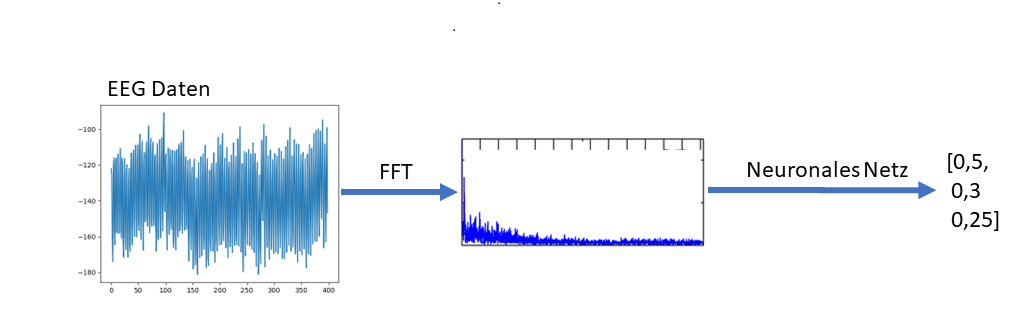
\includegraphics[width=1.0\linewidth]{pictures/Workflow.png}
%     \caption{Zuerst nehmen wir die EEG Daten auf. Danach werden die Daten mit FFT weiterverarbeitet. Die Ergebnisse dieser FFT werden dann an ein neuronales Netzwerk weitergegeben, welches dann die Wahrscheinlichkeiten, die das Netzwerk den einzelnen "Labels" für diesen Datensatz zugeordnet hat, inform eines Vektors ausgibt.}
%     \label{Workflow}
% \end{figure}

% \begin{figure}
%     \centering
%     \begin{tikzpicture}[
%         inputs/.style = {
%             rectangle, draw=black, thick,
%             rotate=90
%         },
%         conv/.style 2 args={
%             rectangle, draw=#2, thick,
%             rotate=#1,
%         },
%         dim/.style = {}
%     ]
%         \node[inputs] (input_layer) {Eingabeschicht};
%         \node[dim, above=0cm of input_layer, rotate=90] {60};
%         \node[dim] at ($(input_layer) + (0,2cm)$) {16};
%         \node[conv={45}{red}, below=1cm of input_layer] {test};
%     \end{tikzpicture}
%     \caption{Caption}
%     \label{fig:my_label}
% \end{figure}

% Unser Ziel war es, ein Framework zu entwickeln, das einfach zu benutzen ist und einem Zeit bei der Entwicklung von BCIs erspart. Dafür haben wir ein eigenes Julia-Package geschrieben, mit dem man einfach Daten aufnehmen und speichern sowie ein eigenes neuronales Netzwerk erstellen und in einer Live-Anwendung testen kann.

% Dieses Package haben wir anschließend getestet, indem wir es genutzt haben, um ein BCI zu entwickeln, welches erkennen kann, ob man gerade an die Richtung rechts oder an die Richtung links denkt. Wie der Klassifizierungsverfahren genauer funktioniert sieht man in \ref{Workflow}. Diese Klassifizierung ist relativ komplex, da dabei kein einfacher Ausschlag oder Anstieg einer bestimmten Frequenz verursacht wird, anders als z.B. beim Blinzeln oder einem akustischem Signal. Deswegen ist es für einen Menschen auch fast unmöglich, nur anhand der Daten des EEGs manuell festzustellen, ob eine Person gerade an eine bestimmte Richtung denkt.

%Um herauszufinden, ob es überhaupt möglich ist mit unserem EEG, das nur 4 Elektroden besitzt, Gedanken an verschiedene Richtungen zu klassifizieren, haben wir zuerst ein neuronales Netz mit Daten, die wir im Internet gefunden haben, trainiert. Diese Daten wurden mit einem 16 Elektroden EEG aufgenommen. Nachdem wir unser Modell mit diesen Daten trainiert haben, haben wir eigene Daten aufgenommen, um zu testen, ob sich dieses Modell auch auf Daten generalisieren lässt, die mit unserem EEG aufgenommen wurden.

% Zuerst haben wir unser Netzwerk mit Daten aus dem Internet trainiert, die von einem EEG mit 16 Elektroden aufgenommen wurden, da wir wissen, dass es möglich ist ein neuronales Netzwerk zu trainieren, das diese Daten klassifizieren kann. Dadurch können wir das Framework von unserer Hardware getrennt testen und so vorläufig eine mögliche Fehlerquelle ausschließen.

\subsection{Das neuronale Netzwerk}

Wir waren in der Lage, eine sehr gute Genauigkeit beim Testen des Modells mit Trainingsdaten zu erreichen. 
% TODO: Graph? Zahlen?
Mit der Genauigkeit ist gemeint, welchen Anteil der gegebenen Datensätze das neuronale Netzwerk korrekt klassifizieren konnte. 
Da die Trainingsdaten dem Modell durch das Trainieren jedoch bereits bekannt waren, haben wir zusätzlich noch die Genauigkeit des Modells bei der Analyse der Testdaten bestimmt. 
Diese wurden vorher nie zum Trainieren des Netzwerks verwendet und repräsentieren somit viel besser die Genauigkeit des Modell in der späteren Verwendung, wo das Modell mit unbekannten, neuen Umständen und neuen, noch nie zuvor gesehenen Daten klarkommen muss.
Bei der Evaluierung des Modells mit Testdaten konnten wir eine Genauigkeit von bis zu ungefähr 44,57\% erreichen (s. Abb. \ref{fig:test_verlauf}). 

\begin{figure}[h!]
    \centering
    \begin{tikzpicture}
        \begin{axis}[
            height=6.5cm,
            width=15cm,
            xlabel={Trainingszeit in s}, 
            ylabel={Testdatengenauigkeit in \%},
            legend pos = north east,
            font = \small
        ]
            \newcommand{\sentMark}{triangle*}
            \newcommand{\gangMark}{}
            % \addplot table [
            %     x expr={\thisrow{Step}*10}, 
            %     y expr={\thisrow{Value}*100}, % dezimal zu Prozent
            %     col sep=comma] {models/TestdataGanglion/OneFile/allConv_4c_1_e0.0005_2023-01-14_17-08-34.csv};
            \addplot+[mark=\sentMark] table [
                x expr={\thisrow{Step}*10}, 
                y expr={\thisrow{Value}*100}, % dezimal zu Prozent
                col sep=comma] {models/TestdataSentdex/OmegaA_16c_sentdex_e1.0e-5_2023-01-14_19-17-21.csv};
            \addplot+[mark=\sentMark] table [
                x expr={\thisrow{Step}*10}, 
                y expr={\thisrow{Value}*100}, % dezimal zu Prozent
                col sep=comma] {models/TestdataSentdex/OmegaA_16c_sentdex_e1.0e-5_2023-01-14_19-23-25.csv};
            \addplot+[mark=\sentMark] table [
                x expr={\thisrow{Step}*10}, 
                y expr={\thisrow{Value}*100}, % dezimal zu Prozent
                col sep=comma] {models/TestdataSentdex/OmegaA_16c_sentdex_e1.0e-5_2023-01-14_20-35-21.csv};
            \addplot+[mark=\sentMark] table [
                x expr={\thisrow{Step}*10}, 
                y expr={\thisrow{Value}*100}, % dezimal zu Prozent
                col sep=comma] {models/TestdataSentdex/OmegaA_16c_sentdex_e5.0e-5_2023-01-14_20-29-09.csv};
            \addplot+[mark=\gangMark, dashed] table [
                x expr={\thisrow{Step}*10}, 
                y expr={\thisrow{Value}*100}, % dezimal zu Prozent
                col sep=comma] {models/TestdataGanglion/OneFile/allConv_4c_1_2023-01-14_16-51-37.csv};
            \addplot+[mark=\gangMark, dashed] table [
                x expr={\thisrow{Step}*10}, 
                y expr={\thisrow{Value}*100}, % dezimal zu Prozent
                col sep=comma] {models/TestdataGanglion/OneFile/allConv_4c_1_e0.0005_2023-01-14_17-49-13.csv};
            \addplot+[mark=\gangMark, dashed] table [
                x expr={\thisrow{Step}*10}, 
                y expr={\thisrow{Value}*100}, % dezimal zu Prozent
                col sep=comma] {models/TestdataGanglion/OneFile/allConv_4c_1_e0.0005_2023-01-14_17-08-34.csv};
            \legend{Testdaten von Sentdex,,,, eigene Testdaten};
        \end{axis}
    \end{tikzpicture}
    \caption{Die Testdatengenauigkeit des in Abb. \ref{fig:netz_struktur} dargestellten Netzwerks im Verlauf. Die durchgezogenen Linien mit Dreiecken repräsentieren die Genauigkeit mit den Testdaten von Sentdex, die gestrichelten Linien die Genauigkeit mit unseren eigenen Testdaten, die mit dem Ganglion aufgenommen wurden. Der unterschiedliche Verlauf der Linien gleichen Typs kommt daher, dass das Netzwerk beim Erstellen mit zufälligen Gewichten initialisiert wird und somit immer einen anderen Verlauf hat.}
    \label{fig:test_verlauf}
\end{figure}

Da wir drei verschiedene Kategorien von Daten nutzen (Gedanken an Rechts, Gedanke an Links und Gedanken weder Rechts noch Links), würde eine zufällige Klassifizierung der Daten zu einer Genauigkeit von 33\% führen.

% Man kann also festhalten, dass es möglich ist, mit unserem Framework ein BCI zu entwickeln, das die Daten, die wir online gefunden haben, deutlich besser als zufällig klassifizieren kann.

Die Struktur des Netzwerks, mit dem wir dies erreicht haben, ist in Abb. \ref{fig:netz_struktur} zu sehen.
Wir haben die Struktur größtenteils mit \eng{trial and error} ermittelt und die in \nameref{section:overfitting} beschriebenen Verfahren genutzt.

\begin{figure}[h!]
    \centering
    \begin{tikzpicture}[
        layer/.style={rotate=90, right=\layersep of #1.south, anchor=north, align=center}
        % baselayer/.style={},
    ]
        \def\layersep{0.4cm};
        \newcommand{\arr}{edge[-stealth]}
        \newcommand{\layerDesc}[2]{\textbf{#1}, {#2}}
        \newcommand{\layerDescB}[2]{\textbf{#1} \\ {#2}}

        \node[rotate=90, anchor=north, align=center] (conv1) {\layerDescB{1D Conv}{$\textrm{Dim}_K$ = 3, Kanäle = 64}};
        \node[layer=conv1] (drop1) {\layerDesc{Dropout}{$P = 20\%$}};
        \node[layer=drop1] (maxpool1){\layerDesc{Max Pool}{$n = 2$}};
        \node[layer=maxpool1] (conv2) {\layerDescB{1D Conv}{$\textrm{Dim}_K$ = 2, Kanäle = 32}};
        \node[layer=conv2] (maxpool2) {\layerDesc{Max Pool}{$n = 2$}};
        \node[layer=maxpool2] (conv3) {\layerDescB{1D Conv}{$\textrm{Dim}_K$ = 2, Kanäle = 16}};
        \node[layer=conv3] (maxpool3) {\layerDesc{Max Pool}{$n=2$}};
        \node[layer=maxpool3] (flatten) {Flatten};
        \node[layer=flatten] (drop2) {\layerDesc{Dropout}{P = 20\%}};
        \node[layer=drop2] (dense1) {\layerDescB{Fully Connected}{Neuronen = 16}};
        \node[layer=dense1] (dense2) {\layerDescB{Fully Connected}{Neuronen = 16}};
        \node[layer=dense2] (dense3) {\layerDescB{Fully Connected}{Neuronen = 64}};
        \node[layer=dense3] (dense4) {\layerDescB{Fully Connected}{Neuronen = 16}};
        \node[layer=dense4] (dense5) {\layerDescB{Fully Connected}{Neuronen = 3}};
        \draw[-stealth]
            (conv1) \arr (drop1)
            (drop1) \arr (maxpool1)
            (maxpool1) \arr (conv2)
            (conv2) \arr (maxpool2)
            (maxpool2) \arr (conv3)
            (conv3) \arr (maxpool3)
            (maxpool3) \arr (flatten)
            (flatten) \arr (drop2)
            (drop2) \arr (dense1)
            (dense1) \arr (dense2)
            (dense2) \arr (dense3)
            (dense3) \arr (dense4)
            (dense4) \arr (dense5)
            ;
    \end{tikzpicture}
    \caption{Struktur von unserem aktuell besten neuronalen Netzwerk. $\textrm{Dim}_K$ steht für die Größe des Kernels, 1d Conv für eine 1-dimensionale Convolutional Schicht.}
    \label{fig:netz_struktur}
\end{figure}

Nachdem wir dieses Teilziel erreicht hatten, wollten wir unser Framework mit Daten testen, die wir selber aufgenommen hatten. 
Dafür haben wir zuerst das EEG von OpenBCI genutzt, da unser eigenes noch nicht fertig war.
% wir es schon verwendet haben und wissen, das es gute EEG Daten liefern kann. 
Da wir noch keine Zeit dafür hatten, konnten wir nicht genug Trainingsdaten aufnehmen, um das Netzwerk effektiv trainieren zu könnnen, da hierfür viele Datensätze benötigt werden.
Also haben wir die EEG-Daten von Sentdex zum Trainieren und unsere selbst aufgenommenen zum Testen verwendet und konnten tatsächlich eine Testdatengenauigkeit von bis zu 43\% erreichen (s. Abb. \ref{fig:test_verlauf}).
Dies ist zwar weit von ideal, aber dennoch sehr beeindruckend, da die Bedingungen von Trainings- und Testdaten so verschieden sind:
Die Daten wurden mit verschiedenen Geräten, von verschiedenen Personen verschiedenen Alters auf verschiedene Weise aufgenommen.
Dies unterstützt unsere Vermutung, dass es auch mit unserer Hardware möglich ist ein BCI zu entwickeln, dass Gedanken an verschiedene Richtungen sicher erkennen kann, da das neuronale Netzwerk bereits ein Kern-Muster, welches wirklich nur mit dem Gedanken zusammenhängt, gefunden hat.


\section{Diskussion}

Ziel unseres Projektes war es, ein Framework zu entwickeln, welches sich leicht auf die eigenen Zwecke anpassen lässt und die Entwicklung von BCIs vereinfacht. 
Dies haben wir mit unserem eigenen Package erreicht, da es Entwicklung in einer stark abstrahierten Form ermöglicht.
Wir arbeiten außerdem momentan an einer ausführlichen Dokumentation mit Beispielen und Anleitungen und, anders als letztes Jahr, versuchen wir alle Funktionen, die wir programmieren, mit Beschreibung, Argumenten etc. zu dokumentieren, siehe unsere Dokumentation \cite{BCIInterfaceDocs}.

Wir haben zwei Ziele für die direkte Zukunft.
Das erste hat mit unserem EEG zu tun: 
Wir wollen die Qualität der Daten unseres eigenen EEGs testen und diese sowie die erreichbare Genauigkeit des neuronalen Netzwerks mit den kommerziellen Versionen vergleichen.
Zweitens wollen wir die Standardwerte verbessern und neue Funktionen implementieren, da wir zwar eine 44,57\% Testdatengenauigkeit erreichen konnten, aber wissen, dass 60\% möglich sind.

Eine wichtige Funktion, die sowohl uns beim Verbessern der Standardwerte als auch Nutzern stark helfen würde, wäre eine Funktion zur Hyperparameter-Optimierung.
Hyperparameter sind bei neuronalen Netzwerken Parameter, die vor dem Trainieren festgelegt werden müssen, wie zum Beispiel die Netzwerkstruktur,  die Velust- und Aktivierungsfunktionen, die Lernrate, die Regularisierungsfunktionen, Pruning, etc. 
Eine Hyperparameter-Optimierung kann automatisch gute Hyperparameter finden, indem sie systematisch verschiedene Konfigurationen ausprobiert und bessere entwickelt.
Eine Hyperparameter-Optimierung würde uns helfen, da wir so schneller bessere Standardwerte finden könnten.
Denn das \eng{Trial and Error} Verfahren, vor allem per Hand, ist sehr zeitaufwändig -- inzwischen haben wir vermutlich schon hunderte verschiedene Konfigurationen manuell erstellt und ausprobiert.
Außerdem würde ein Hyperparamter-Optimierung es erlauben, dass unser Framework in einer noch größeren Anzahl an Szenarien ohne manuelle Anpassung benutzt werden könnte.

Wir haben bereits eine Idee für ein solches Verfahren, welches eine evolutionäres Vorgehensweise nutzen würde:
Das Programm würde unsere Standardkonfiguration (s. \nameref{section:UnsereImplementation}) als Basis nehmen, diese mehrfach kopieren und zufällig abändern, und dann alle Kopien für z.B. 20 Sekunden trainieren.
Danach würde es sich die beste Konfiguration auswählen, diese wieder kopieren und zufällig verändern und den ganzen Prozess erneut beginnen.
Doch wir wollen uns noch weiter mit den verschiedenen möglichen Verfahren beschäftigen und müssen die Hyperparameter-Optimierung natürlich noch implementieren und testen.

Weiter in der Zukunft, nachdem wir hoffentlich mit unserem aktuellen Anwendungsbeispiel eine zufriedenstellende Genauigkeit erreichen konnten, werden wir weitere Anwendungsbeispiele umsetzen und dafür Daten sammeln.
Nur so können wir sichergehen, dass unser Framework am Ende nicht einfach nur für einen Zweck verwendbar ist (s. \nameref{section:UnsereImplementation}).

\newpage

\section{Danksagung}

Danke an den Förderverein \enquote{Gesellschaft der Freunde des Gymnasium Eversten e.V.} für die Finanzierung des EEG-Geräts. Ohne diese Hilfe wäre dieses Projekt nie zustande gekommen. Alle finanzierten Teile sind in der \hyperref[Materialien]{Materialliste} mit $\star$ gekennzeichnet.

Größter Dank geht an unseren Projektbetreuer Herr Dr. Glade, der unser Projekt begleitet hat. 
Er hat uns bei der wissenschaftlichen Methodik geholfen und uns wichtige Ressourcen zur Hand gegeben sowie bei Fragen weitergeholfen.

\section{Quellen}
\subsection{Abbildungen}
\begin{table}[h!]
    % Abstand zwischen Tabellenzeilen
    \renewcommand*{\arraystretch}{1.2}
    \centering
    {
    \setlength{\tabcolsep}{0pt}
    \begin{tabular}{p{0.15\linewidth}p{0.85\linewidth}}
        Abb. \ref{fig:conv_layers} und \ref{fig:conv_layers_channels}%
        & Kopiert und abgeändert von \url{https://tikz.net/conv2d/}, ursprünglicher Author ist Janosh Riebesell  \\
        % Abb. \ref{fig:dense_nn} %
        % & Kopiert und abgeändert von \href{https://tikz.net/regular-vs-bayes-nn/}{https://tikz.net/regular-vs-bayes-nn/}, ursprünglicher Author ist Janosh Riebesell \\
        Abb. \ref{fig:OPV} %
        & Linkes Bild: \url{www.conrad.de/de/ratgeber/handwerk-industrie-wiki/elektronik-bauteile/lm393.html}, rechtes Bild: \url{https://www.reichelt.de/operationsverstaerker-2-fach-dip-8-lm-358-dip-p10483.html} \\
        Abb. \ref{fig:LHP} %
        & Kopiert, ursprünglich erstellt von Józef Król, siehe \url{https://docplayer.pl/48121857-Szybkie-metody-projektowania-filtrow-aktywnych.html} \\
    \end{tabular}
    }
    \label{tab:my_label}
\end{table}

Alle anderen Abbildungen wurden selbst erstellt.

% \subsection{Quellen}
\subsection{Literatur}
\printbibliography[heading=none, title={Literatur}, keyword={Literatur}]
\subsection{GitHub-Repositories und Videos}
\printbibliography[heading=none, title={Anderes}, notkeyword={Literatur}]
\end{document}